\documentclass{article}

\usepackage{colt11e}
\usepackage[round,comma]{natbib}
\usepackage{amssymb,amsmath,mathrsfs}
\usepackage{graphicx}
\usepackage[all]{xy}
\usepackage[ruled,section]{algorithm}
\usepackage[noend]{algorithmic}
\bibliographystyle{plainnat}
\let\cite\citep

\makeatletter
\def\cL{{\mathscr L}}
\def\cB{{\mathscr B}}
\def\cK{{\mathscr K}}
\def\cR{{\mathscr R}}
\def\cN{{\mathcal N}}
\def\cM{{\mathcal M}}
\def\RC{{\mathcal R}}
\def\fF{\mathfrak{F}}
\def\fI{\mathfrak{I}}
\def\fM{\mathfrak{M}}
\def\AA{A}
\def\RR{\mathbb{R}}
\def\NN{\mathbb{N}}
\def\ZZ{\mathbb{Z}}
\def\DD{\mathbb{D}}
\def\LL{\mathbb{L}}
\def\YY{\mathbb{Y}}
\def\XX{\mathbb{X}}
\newcommand{\XXX}{{\mathscr X}}
\newcommand{\XXell}{[\XX]^\ell}
\newcommand{\X}{\bar X}
\newcommand{\x}{\bar x}
\renewcommand{\geq}{\geqslant}
\renewcommand{\leq}{\leqslant}
\renewcommand{\emptyset}{\varnothing}\newcommand{\emset}{\varnothing}
\renewcommand{\kappa}{\varkappa}
\renewcommand{\phi}{\varphi}
\renewcommand{\epsilon}{\varepsilon}\newcommand{\eps}{\varepsilon}
\renewcommand{\lim}{\mathop{\operator@font lim}\limits}
\renewcommand{\limsup}{\mathop{\operator@font lim\,sup}\limits}
\renewcommand{\liminf}{\mathop{\operator@font lim\,inf}\limits}
\renewcommand{\max}{\mathop{\operator@font max}\limits}
\renewcommand{\min}{\mathop{\operator@font min}\limits}
\renewcommand{\sup}{\mathop{\operator@font sup}\limits}
\renewcommand{\inf}{\mathop{\operator@font inf}\limits}
\newcommand{\argmin}{\mathop{\operator@font arg\,min}\limits}
\newcommand{\argmax}{\mathop{\operator@font arg\,max}\limits}
\newcommand{\Arg}{\mathop{\rm Arg}\limits}
\newcommand{\Argmin}{\mathop{\rm Arg\,min}\limits}
\newcommand{\Argmax}{\mathop{\rm Arg\,max}\limits}
\newcommand{\diag}{\mathop{\mathrm{diag}}}
\newcommand{\sign}{\mathop{\rm sign}\limits}
\newcommand{\const}{\mathrm{const}}
\newcommand{\conv}{\mathrm{conv}}
\newcommand{\KL}{\mathrm{KL}}
\newcommand{\VCdim}{\mathop{\mathrm{VCdim}}\nolimits}
\newcommand{\scal}[2]{\left\langle #1,#2 \right\rangle}
\newcommand{\what}{\widehat}
\newcommand{\wtil}{\widetilde}
\newcommand{\eqdef}{\equiv}
\def\CC_#1^#2{\tbinom{#1}{#2}}
%\def\CC_#1^#2{C_{#1}^{#2}}
\providecommand{\Prob}{\mathsf{P}}
\def\Pr[#1]{\Prob\left[#1\right]}
\def\Prbig[#1]{\Prob\bigl[#1\bigr]}
\def\PrBig[#1]{\Prob\Bigl[#1\Bigr]}
\newcommand{\Expect}{\mathsf{E}}
\newcommand{\Var}{\mathsf{D}}
\newcommand{\bin}{\mathop{\rm bin}\nolimits}
\newcommand{\Bin}{\mathop{\rm Bin}\nolimits}
\newcommand{\hypergeom}[5]{{#1}_{#2}^{#4,\:#3}\left(#5\right)}
\newcommand{\hyper}[4]{\hypergeom{h}{#1}{#2}{#3}{#4}}
\newcommand{\Hyper}[4]{\hypergeom{H}{#1}{#2}{#3}{#4}}
\newcommand{\HyperR}[4]{\hypergeom{\bar{H}}{#1}{#2}{#3}{#4}}

% for algorithms
\newcommand{\IFTHEN}[1]{\STATE\algorithmicif\ #1 {\algorithmicthen}}
\newcommand{\REMARK}[1]{\item[]\textsl{#1}}
\newcommand{\BEGIN}{\\[1ex]\hrule\vskip 1ex}
\newcommand{\END}{\vskip 1ex\hrule\vskip 1ex}
\newcommand{\EXIT}{\STATE\textbf{exit}}
\newcommand{\vkID}[1]{\text{\sf #1}}
\newcommand{\PROCEDURE}[1]{\medskip\STATE\textbf{Procedure} \vkID{#1}}

\def\XYtext(#1,#2)#3{\rlap{\kern#1\lower-#2\hbox{#3}}}
\newcommand{\TODO}[1]{\par\smallskip\noindent\fbox{\parbox{150mm}{\textsf{\textbf{~~TO DO:} #1}}}\par\smallskip}
\makeatother

%%%%%%%%%%%%%%%%%%%%%%%%%%%%%%%%%%%%%%%%%%%%%%%%%%%%%%%%%%%%%%%
% Author's hacking for SLANTED THEOREMS -- may be removed
\makeatletter
\def\@begintheorem#1#2{\trivlist
   \item[\hskip \labelsep{\bfseries #1\ #2}]\slshape}
\def\@opargbegintheorem#1#2#3{\trivlist
      \item[\hskip \labelsep{\bfseries #1\ #2\ (#3)}]\slshape}
\def\@endtheorem{\endtrivlist}
\renewcommand{\emph}[1]{\textit{#1}}
\makeatother
% The END of "Author's hacking"
%%%%%%%%%%%%%%%%%%%%%%%%%%%%%%%%%%%%%%%%%%%%%%%%%%%%%%%%%%%%%%%%

\newtheorem{conjecture}[theorem]{Conjecture}
\newtheorem{remark}[theorem]{Remark}
\newenvironment{proofsketch}{\noindent{\bf Proof sketch:}}{\qed\medskip}

\title{%
    Combinatorial generalization bounds%
    %Splitting and connectivity generalization bounds%
    %Combinatorial generalization bounds based on both splitting and connectivity properties of the set of classifiers%
    %Combinatorial theory of overfitting%
    %Combinatorial nature of learning%
    \thanks{Supported by Russian Foundation for Basic Research
        grants 08-07-00422, 11-07-00480 and the program
        ``Algebraical and combinatorial methods of cybernetics and new generation information systems''
        of Russian Academy of Sciences, Branch of Mathematical Sciences.}
}

\author{
    K. V. Vorontsov\\
    Computing Center RAS\\
    \texttt{\small voron@forecsys.ru}
\And
    A. A. Ivahnenko\\
    Moscow Institute \\of Physics and Technology\\
    \texttt{\small ivahnenko@forecsys.ru}
\And
    P. V. Botov\\
    Moscow Institute \\of Physics and Technology\\
    \texttt{\small pbotov@forecsys.ru}
\AND
    I. M. Reshetnyak\\
    Moscow State University\\
    \texttt{\small ilya.reshetnyak@gmail.com}
\And
    I. O. Tolstikhin\\
    Computing Center RAS\\
    \texttt{\small iliya.tolstikhin@gmail.com}
}

\begin{document}
\maketitle

\begin{abstract}
    In this paper we propose a new combinatorial technique
    for obtaining data dependent generalization bounds.
    We~introduce a~splitting and connectivity graph (SC-graph) over the set of classifiers.
    In~some cases the knowledge of this graph leads to an exact generalization bound.
    Typically, the knowledge of a~little part of the SC-graph is~sufficient
    for reasonable approximation of the bound.
    Being applied to a parametric set of conjunctive rules our bound
    helps to obtain more reliable classifiers as compositions of less overfitted rules.
\end{abstract}

\section{Introduction}

The accurate bounding of overfitting %generalization ability
remains one of the most challenging open problems in computational learning theory
starting with VC-theory~\cite{vapnik71uniform-eng}.
Generalization bounds are still pessimistically overestimated
regardless of recent significant improvements, see surveys
\cite{vayatis99distributiondependent,langford02quantitatively,boucheron05theory}.
Conservative bounds are not always suitable for overfitting understanding, prediction, and control.
Another difficulty is~that both final and intermediate bounds
are usually expressed in terms of unobservable quantities.
Therefore it is not always possible to measure and compare the factors of overestimation.
For~classical VC~bounds
such empirical measurement has been performed in~\cite{voron08pria-eng}.
The~permutational probability framework has been developed
to make intermediate bounds measurable.
It~has been shown that overfitting depends
not only on the number of different classifiers (shattering coefficient)
but in~greater degree on their diversity.
Splitting and connectivity properties of the set of classifiers are two aspects of diversity
that reduce overfitting and might help to obtain tighter~bounds.

The \emph{splitting} property means that
only a~small part of classifiers from a~given set have a low error rate
and, as a~result, a~high chance to~be produced by~a~learning algorithm.
Splitting happens when we~deal with a certain problem having a~fixed target function.

The \emph{connectivity} property means that
for~any classifier from a~given parametric set there exist
a~number of classifiers from the set differing from the first one by exactly one object.
Such classifiers are called \emph{connected}.
Connectivity owes to parameter continuity of a~classification function.

Experiments with split and non-split chains of classifiers~\cite{voron09roai2008}
showed that the absence of one of these advantageous properties
can result in significant overfitting
even though the set contains a~few dozens of classifiers.
Hence, to possess both splitting and connectivity properties is a must for sets containing billions of classifiers in practice.

In~this work we develop a~combinatorial theory
that accurately deals with both splitting and connectivity
and gives tight or even exact bounds on probability of overfitting.
Basic definitions and notations are introduced in section~\ref{sec:Defs}.
Section~\ref{sec:FC&VC}
    revisits two classical bounds in terms of permutational probabilities.
In~section~\ref{sec:ProtProh}
    we introduce the principle of~protective and prohibitive subsets
    fundamental for further considerations.
Section~\ref{sec:SC-bound}
    contains main theorems about splitting and connectivity (SC) bounds.
In~section~\ref{sec:ModelSets}
    we show that SC-bounds can be exact for some nontrivial sets of classifiers.
In~section~\ref{sec:RuleLearning}
    then SC-bound is applied to the set of conjunctive rules.
    The overfitting reduction strategy is~proposed
    that can be easily incorporated into existing rule induction engines.
    The experiment shows that the usage of SC-bound results in better generalization on real data sets.

%Obtaining exact generalization bounds remains an open problem in
%Computational Learning Theory~\cite{boucheron05theory}.
%Experiments~\cite{voron08pria-eng,voron09roai2008} have shown that
%to~obtain exact bounds, one should simultaneously take into account two fine effects:
%the \emph{splitting} of the set into error levels and the similarity of classifiers.
%Many practically used sets contain a lot of extremely similar classifiers
%that differ only on one object, we call them \emph{connected}.
%Taking into account the effects of splitting and connectivity can give
%very tight or even exact generalization bounds.
%We~apply a new SC (splitting and connectivity) bound to the set of conjunctive rules
%and propose the overfitting reduction method compatible with many standard rule induction engines.

\section{Definitions and notation}
\label{sec:Defs}

Let $\XX=\{x_1,\ldots,x_L\}$  be a set of objects and
$A$ be a set of classifiers.
By~$I\colon A\times X \to \{0,1\}$ denote a~binary loss function such that
$I(a,x)=1$ if a~classifier~$a$ produces an~error on an~object~$x$.
For~further considerations there is no need to specify what is ``classifier''.
Particularly, regression function can also be a~``classifier''
if a~binary loss function is~used.

\medskip
A~binary vector $(a_i)\equiv\bigl(I(a,x_i)\bigr){}_{i=1}^L$
of size~$L$ is called an \emph{error vector} of the classifier~$a$.
Assume that all classifiers from~$A$ have pairwise different error vectors.
The number of errors of a~classifier~$a$ on a~sample $X\subseteq\XX$
is defined as $n(a,X) = \sum_{x\in X} I(a,X)$.
Denote $n(a)=n(a,\XX)$ for short.
The~error rate is defined as
$\nu(a,X) = \frac1{|X|} n(a,X)$.
A \emph{learning algorithm} is a mapping ${\mu\colon 2^\XX \to A}$
that takes a~training sample~$X\subseteq\XX$  and gives a classifier ${\mu X \in A}$.

\paragraph{Permutational (transductive) probability.}
By $\XXell$ denote a set of all
$\CC_L^\ell = \tfrac{L!}{\ell!(L-\ell)!}$
samples $X\subset\XX$ of size~$\ell$.
Assume that all partitions of the set $\XX$ into
an observed training sample~$X$ of size~$\ell$
and a hidden test sample $\X=\XX\setminus X$ of size~$k=L-\ell$
can occur with equal probability.

If~the \emph{discrepancy}
$\delta(a, X) = \nu(a,\X) - \nu(a, X)$
is~greater than a~given nonnegative threshold~$\eps$,
then the classifier~$a=\mu X$ is said to be \emph{overfitted}.
Our goal is to estimate the \emph{probability of overfitting}:
\[
    Q_\eps (\mu, \XX)
    =
    \Prob\bigl[
        \delta(\mu, X) \geq \eps
        %\nu(\mu X,\X) - \nu(\mu X, X) \geq \eps
    \bigr]
    =
    \frac 1{\CC_L^\ell} \sum_{X\in\XXell}
    \bigl[
        \delta(\mu,X) \geq \eps
    \bigr].
\]
where
$\delta(\mu, X) = \delta(\mu X, X)$ for short;
the square brackets denote a transformation of a~logical value into numerical  one
according to Iverson's convention:
$[\textit{true}]=1$, $[\textit{false}]=0$~\cite{knuth98concrete-eng}.

The \emph{inversion} of an~upper bound $Q_\eps \leq \eta(\eps)$  is an inequality
$\nu(\mu X,\X) \leq \nu(\mu X, X) + \eps(\eta)$
that holds with probability at least $1-\eta$, where $\eps(\eta)$
is the inverse function for $\eta(\eps)$.

\medskip
The permutational probabilistic framework seems to be restrictive because
the fundamental notion of ``probability'' degenerates into the trivial ``fraction of partitions''.
Nevertheless, the  independence assumption is~actually kept in~this framework.
This is quite sufficient to~derive
the law of large numbers, rank tests, VC-bounds, and many other fundamental statistical facts.

\medskip
The permutational framework has three advantages:

1) it~makes redundant some usual intermediate bounds as~symmetrization~\cite{philips05datadependent};

2) it~allows to measure probabilities empirically in a~manner of~cross-validation;

3) it~encourages~us to~keep bounds in~exact, non-asymptotical form.

\paragraph{Learning algorithms.}%
\emph{Empirical risk minimization} (ERM) is a~classical and perhaps most natural example of~the learning algorithm:
\begin{equation}
\label{ERM}
	 \mu X \in A(X) = \Arg\min_{a\in A} n(a,X).
\end{equation}

The choice of a classifier minimizing empirical risk may be ambiguous
because of the discreteness of the function $n(a,X)$.
ERM algorithm $\mu$ is said to be \emph{pessimistic} or \emph{optimistic} if, respectively,
\[
    \mu X = \arg\max_{a\in A(X)} n(a,\X);
    \qquad
    \mu X = \arg\min_{a\in A(X)} n(a,\X).
\]

The \emph{probability $\wtil Q_\eps$ of a large uniform deviation}
is~considered as a~main functional to be bounded
in Vapnik-Chervonenkis and Rademacher Complexity theories of generalization:
\begin{equation}
\label{eq:Quniform}
    Q_\eps(\mu, \XX)
    \leq
    \wtil Q_\eps(A, \XX)
    \eqdef
    \Prob
    \Bigl[
        \max_{a\in A} \delta(a,X) \geq \eps
    \Bigr].
\end{equation}

The uniform functional $\wtil Q_\eps$ can give highly overestimated upper bounds on~$Q_\eps$.
Nevertheless, it is widely used because its bounds hold for any learning algorithm~$\mu$.
Minimizing the inversion of~a~bound leads
to a~new learning algorithm that tends to~reduce overfitting, by construction.
This is a~standard way to get practical outcome from generalization bounds.
A~number of complexity penalization methods has been obtained
in this way~\cite{vapnik98stat,langford02quantitatively}.

The uniform functional $\wtil Q_\eps$ can also be represented as a probability of~overfitting
for a~special learning algorithm called \emph{discrepancy maximization}:
\[
    \mu X = \arg\max_{a\in A} \delta(a,X).
\]

The~pessimistic ERM, optimistic ERM, and discrepancy maximization cannot be implemented in~practice
because they look into a~hidden part of~data~$\X$ unknown at the~learning stage.
Nevertheless, they are very useful for theoretical considerations because of the following relationships.

\begin{lemma}
\label{lem:relationships}
    For any set $\XX$ and any ERM learning algorithm~$\mu$
    \[
        Q_\eps(\mathrm{OptERM}, \XX)
        \leq
        Q_\eps(\mu, \XX)
        \leq
        Q_\eps(\mathrm{PessERM}, \XX)
        \leq
        Q_\eps(\mathrm{DiscrMax}, \XX)
        =
        \wtil Q_\eps(A, \XX).
    \]
\end{lemma}

\section{Fixed classifier bound and Vapnik-Chervonenkis bound}
\label{sec:FC&VC}

In this section we show that permutational probabilistic framework
gives an exact bound for a~fixed classifier (FC) and an upper Vapnik-Chervonenkis (VC) bound
by a~quite straightforward way.

\paragraph{Hypergeometric distribution.}
For a~classifier~$a$ such that $m=n(a,\XX)$
the probability to~have $s$~errors on a~sample~$X$
is~given by a~hypergeometric function:
\[
    \Prbig[ n(a,X)=s ]
    =
    \Prbig[ n(a,\X)=m-s ]
    =
    \hyper{L}{m}{\ell}{s},
\]
where
$\hyper{L}{m}{\ell}{s} = {\CC_m^s \CC_{L-m}^{\ell-s}} / {\CC_L^\ell}$,
argument~$s$ runs from~${s_0 = \max\{0,m-k\}}$ to ${s_1 = \min\{m,\ell\}}$,
parameter~$m$ takes values $0,\ldots,L$.
It is assumed that
$\CC_m^s = \hyper{L}{m}{\ell}{s} = 0$
for all other integers $m,s$.

Define the cumulative distribution function (left tail) of the hypergeometric distribution
%\begin{equation}
%\label{eqHypergeometric}
\[
    \Hyper{L}{m}{\ell}{z}
    =
    \sum\limits_{s=s_0}^{\lfloor z \rfloor}
    \hyper{L}{m}{\ell}{s}.
\]
%\end{equation}

Consider a~set $A=\{a\}$ containing only a~fixed classifier, so that $\mu X = a$ for any $X$.
Then the probability of overfitting~$Q_\eps$ transforms into
the probability of~large deviation between error rates on two samples~$X,\X$.
If~the number of errors $n(a)$ is~known, then an~exact $Q_\eps$ bound can be obtained.

\begin{theorem}[FC-bound]
\label{thOneAlg}
    For any set $\XX$,
    any $\eps\in [0,1]$,
    and a~fixed classifier~$a$ such that ${m=n(a)}$
    the probability of~overfitting is~given by the left tail of the hypergeometric distribution:
    \begin{equation}
    \label{eq:OCbound}
        Q_\eps(a, \XX)
        %\Prbig[ \delta(a,X) \geq \eps ]
        =
        \Hyper{L}{m}{\ell}{ \tfrac{\ell}{L} (m-\eps k) }.
    \end{equation}
\end{theorem}
\begin{proof}
    Denote ${s=n(a,X)}$ and rewrite the overfitting condition
    ${\delta(a,X) \geq \eps}$
    as
    $\tfrac1k (m-s) - \tfrac{1}{\ell} s \geq \eps$
    or equivalently
    ${s \leq \tfrac{\ell}{L} (m-\eps k) \eqdef s_m(\eps) }$. Then
    \[
        Q_\eps
        =
        \Prob\bigl[
            n(a,X) \!\leq\! s_m(\eps)
        \bigr]
        =
        \sum\limits_{s=s_0}^{\lfloor s_m(\eps) \rfloor}
        \Prob\bigl[
            n(a,X) \!=\! s
        \bigr]
        =
        \sum\limits_{s=s_0}^{\lfloor s_m(\eps) \rfloor}
        \hyper{L}{m}{\ell}{s}
        =
        \Hyper{L}{m}{\ell}{ s_m(\eps) }.
    \]
    \vskip-3ex
\end{proof}

The hypergeometric distribution plays a fundamental role in all further combinatorial bounds.

\begin{theorem}[VC-bound]
\label{thOneAlg}
    For any set $\XX$,
    any learning algorithm~$\mu$,
    and any $\eps\in [0,1]$
    the probability of~large uniform deviation is bounded by the sum of FC-bounds over the set~$A$:
    \begin{equation}
    \label{eq:VCbound}
        %Q_\eps(\mu, \XX)
        \wtil Q_\eps(A, \XX)
        %\Prbig[ \delta(a,X) \geq \eps ]
        \leq
        \sum_{a\in A}
        \Hyper{L}{m}{\ell}{ \tfrac{\ell}{L} (m-\eps k) },
        \quad
        m = n(a).
    \end{equation}
\end{theorem}
\begin{proof}
    %Apply a union bound which is in fact a substitute of binary values sum for their maximum:
     Apply a union bound substituting the maximum of binary values by their sum:
    \[
        \wtil Q_{\eps} =
        \Prob
        \max_{a\in A}
        \bigl[
            \delta(a,X) \!\geq\! \eps
        \bigr]
        \leq
        \sum_{a\in A}
        \Prob
        \bigl[
            \delta(a,X) \!\geq\! \eps
        \bigr]
        =
        \sum_{a\in A}
        \Hyper{L}{m}{\ell}{s_m(\eps)},
        \quad
        m = n(a).
    \]
    \vskip-3ex
\end{proof}

The union bound is the only reason of the looseness of the VC-bound~\eqref{eq:VCbound}.

Note that further weakening gives a~well known form of the VC-bound~\cite{vapnik98stat}:
\[
    \wtil Q_\eps(A, \XX)
    \leq
    |A| \max_m \Hyper{L}{m}{\ell}{s_m(\eps)}
    \leq
    |A| \cdot \tfrac32 e^{-\eps^2\ell},
    \quad
    \text{if } \ell=k,
\]
where $|A|$ is~called a \emph{shattering coefficient} of~the set of classifiers~$A$ on~the~set~$\XX$.
%We~will not use it.

\medskip
It is well known that VC-bound is highly overestimated which can be explained by the fact that
all classifiers make approximately equal contributions to the VC-bound.
However, the set of classifiers is usually split into error rates in~quite nonuniform manner.
Most classifiers are bad, therefore,
have vanishing probability to be obtained as a result of learning
and make a~negligible contribution to the probability of overfitting.
On~the~other hand, similar classifiers share their contribution,
thus each of them contributes poorly again.
VC~bound totally ignores these advantageous effects.
The uniform deviation bound sacrifices the splitting effect;
the union bound sacrifices the similarity effect.

\medskip
Note that the initial proof by Vapnik and Chervonenkis was purely combinatorial.
Later %in~search of~more accurate bounds
a~combinatorial approach was neglected in~favor~of more sophisticated techniques from
functional analysis and concentration of~measure~\cite{lugosi98concentrationmeasure,boucheron00sharp}.
We~wish revisit this point and demonstrate that the combinatorial approach
has not exhausted its potential.

\section{The principle of protective and prohibitive subsets}
\label{sec:ProtProh}

The principle of protective and prohibitive sets~\cite{voron10pria-eng}
is based on the conjecture that
the necessary and sufficient condition for $\mu X=a$ can be specified explicitly
for any classifier $a\in A$
in~terms of subsets of~objects.
From this conjecture an exact $Q_\eps$ bound has been derived.

In~this work we use a similar conjecture relaxed to the necessary condition
and derive an upper bound which has a~simpler form.

\begin{conjecture}
\label{hyp:1}
    For each classifier $a\in A$  there exists
    a~\emph{protective subset} $X_a\in \XX$ and
    a~\emph{prohibitive subset} $X'_a\in \XX$ such that
    for any $X\in\XXell$
    \begin{equation}
    \label{eq:hyp1}
    	\bigl[ \mu X \!=\! a \bigr] \leq
        \bigl[X_a \!\subseteq\! X \bigr]
        \bigl[X'_a \!\subseteq\! \X \bigr].
    \end{equation}
\end{conjecture}

The subset $\XX{\setminus} X_a{\setminus} X'_a$
is~called \emph{neutral} for a~classifier~$a$.
The presence or absence of neutral objects in a~training sample~$X$
does not change the result of learning~$\mu X$.
Later we will give nontrivial examples of $\mu$ and $A$ that satisfy conjecture~\ref{hyp:1}.

\begin{lemma}
\label{lem1}
    If conjecture~\ref{hyp:1} holds,
    then the probability to~learn a~classifier~$a$ can be bounded:
    \[
        \Prbig[ \mu X\!=\!a ]
        \leq
        P_a
        \equiv
        {\CC_{L_a}^{\ell_a}} / {\CC_{L}^{\ell}},
    \]
    where
    $L_a = L - |X_a| - |X'_a|$ and
    $\ell_a = \ell - |X_a|$
    are the number of neutral objects for~a~classifier~$a$ in the general set~$\XX$ and sample~$X$ respectively.
\end{lemma}
\begin{proof}
    According to the conjecture
    ${
        \Prbig[ \mu X\!=\!a ]
        \leq
        \Prob
        \bigl[  X_a\subseteq  X \bigr]
        \bigl[ X'_a\subseteq \X \bigr]
    }$.
    The right-hand side
    is a fraction of~partitions ${\XX=X\sqcup\X}$ such that
    ${X_a\subseteq  X}$ and ${X'_a\subseteq  \X}$.
    The number of~such partitions is equal to~$\CC_{L_a}^{\ell_a}$.
    The number of all partitions is equal to~$\CC_{L}^{\ell}$,
    hence their ratio gives~$P_a$.
\end{proof}

\begin{theorem}
\label{th:1}
    If conjecture~\ref{hyp:1} holds, then
    for any $\eps\in[0,1]$
    the bound on probability of overfitting is
    \begin{equation}
    \label{eq:th1}
        Q_\eps
        \leq
        \sum_{a\in \AA} P_a \Hyper{L_a}{m_a}{\ell_a}{s_a(\eps)},
    \end{equation}
    where
    ${m_a = n(a,\XX{\setminus} X_a {\setminus} X'_a)}$
    is a~number of errors that classifier~$a$ produces on~neutral objects and
    ${s_a(\eps) = \tfrac\ell L \bigl( n(a)-\eps k \bigr) - n(a,X_a)}$
    is a~largest number of errors $n(a,X{\setminus}X_a)$
    that classifier~$a$ produces on~neutral training objects
    provided that discrepancy $\delta(a,X)$ exceeds~$\eps$.
\end{theorem}

\begin{proof}
    The probability of~overfitting~$Q_\eps$
    can be found as a total probability
    from probability to~learn each of classifiers $\Prbig[ \mu X\!=\!a ]$
    and conditional probabilities
    ${
        Q_{\eps|a} = \Prbig[ \delta(a,X) \!\geq\! \eps \mid a\!=\!\mu X ]
    }$:
    \[
        Q_\eps
        =
        \sum_{a\in \AA}
            \Prbig[ \mu X\!=\!a ] Q_{\eps|a}
        \leq
        \sum_{a\in \AA}
            P_a Q_{\eps|a}.
    \]
    The conditional probability $Q_{\eps|a}$ can be obtained from theorem~\ref{thOneAlg}
    by~taking into account that
    the subsets $X_a$ and $X'_a$ can not be involved in~partitioning given a~fixed classifier~$a$.
    Only $L_a$~neutral objects are partitioned
    into $\ell_a$~training and $L_a-\ell_a$ testing objects.
    To~employ theorem~\ref{thOneAlg} we~express the discrepancy $\delta(a,X)$
    in~terms or the number of errors on neutral training objects $s = n(a,X{\setminus} X_a)$:
    \[
        \delta(a,X) =
        \tfrac1k \bigl( n(a)-s-n(a,X_a) \bigr) -
        \tfrac1\ell \bigl( s+n(a,X_a) \bigr).
    \]
    Condition $\delta(a,X)\geq \eps$ is~equivalent to $s\leq s_a(\eps)$.
    Then $Q_{\eps|a} = \Hyper{L_a}{m_a}{\ell_a}{ s_a(\eps) }$
    and~\eqref{eq:th1} holds.
\end{proof}

Note that the sum $\sum_a P_a$ can be interpreted
as a~degree of looseness of the bound~\eqref{eq:th1}.
The~bound is~exact if this sum is equal to~1.

\medskip
The principle of protective and prohibitive subsets
is a~powerful tool to~obtain combinatorial generalization bounds.
In~\cite{voron10pria-eng} it has been used to obtain exact bounds on probability of overfitting
for model sets of classifiers like monotonic and unimodal chains.
This work is focused on~common bounds for arbitrary sets of classifiers
that take into account both splitting and connectivity properties of~the~set.

\section{Splitting and connectivity bounds}
\label{sec:SC-bound}

\paragraph{The splitting and connectivity graph.}
Define an order relation on classifiers $a\leq b$ as a natural order over their error vectors:
$a_i \leq b_i$ for all $i=1,\ldots,L$.
Define a~metric on classifiers as a Hamming distance between error vectors:
$\rho(a,b) = \sum_{i=1}^L |a_i-b_i|$.
Classifiers $a$ and $b$ are called \emph{connected} if $\rho(a,b) = 1$.
Define the precedence relation on classifiers $a\prec b$ as
$\bigl(a\leq b\bigr) \wedge \bigl( \rho(a,b)=1 \bigr)$.

%\bigskip
%{\LARGE
%$x_1$ $x_2$ $x_3$ $x_4$ $x_5$ $x_6$ $x_7$ $x_8$ $x_9$ $x_{10}$ }
%\bigskip

The set of classifiers $A$ can be represented by
a~multipartite directed graph $\langle A, E \rangle$
that we call the \emph{splitting and connectivity graph} (SC-graph)
in which vertices are classifiers, and
edges $(a,b)$ are pairs of classifiers such that $a\prec b$,
see example on~Figure~\ref{fig:SC-graph-lin}.
The partite subsets $A_m = \{ a\in A\colon n(a)=m \}$
are called \emph{error layers}, $m=0,\ldots,L$.
Each edge of the SC-graph $(a,b)$ corresponds to an object $x_{ab}\in\XX$
such that $I(a,x_{ab})=0$ and $I(b,x_{ab})=1$.
\begin{figure}[t]
    \noindent\centering
    \raisebox{3mm}{(a)~}
    \includegraphics[width = 60mm]{SimpleSample1num.PNG.eps}
    \qquad
    \raisebox{3mm}{(b)~}
    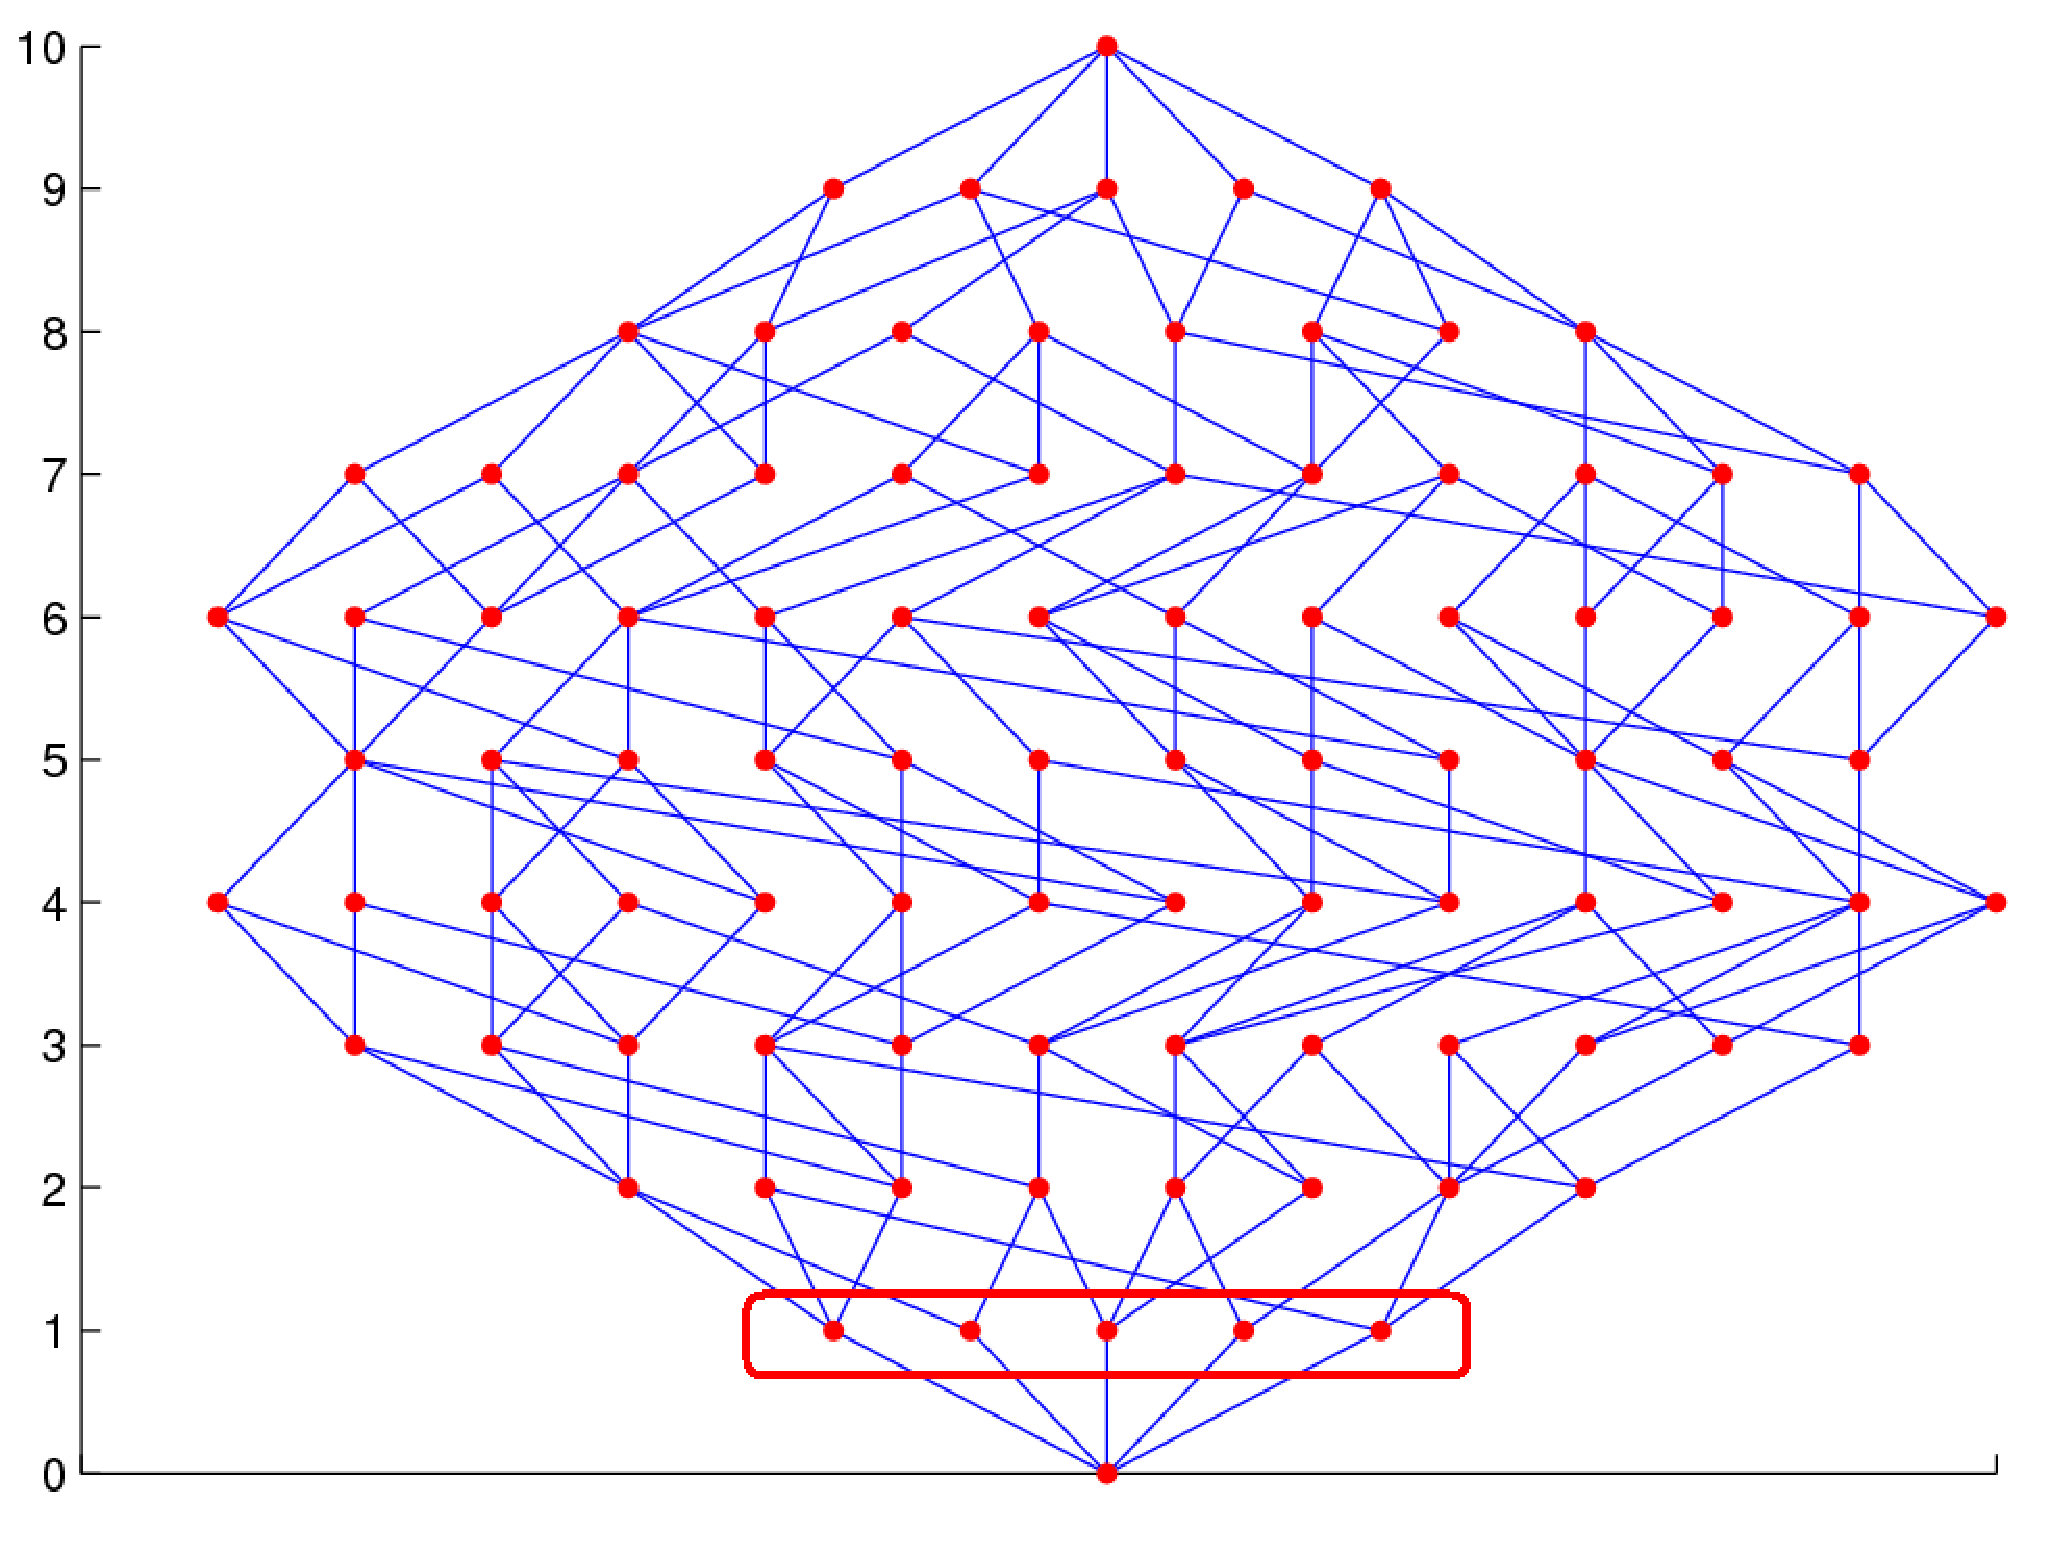
\includegraphics[width = 60mm]{SimpleGraph1.PNG.eps}
    \XYtext(-65mm,43mm){\scriptsize{$m$}}%
    \\\medskip
    \raisebox{-10mm}{(c)}
    \scriptsize
    \begin{tabular}{c|c|ccccc|cccccccc|c}
        & {layer 0} &
        \multicolumn{5}{c|}{layer 1} &
        \multicolumn{8}{c|}{layer 2} \\
        $x_1$ & 0 & 1 & 0 & 0 & 0 & 0 & 1 & 0 & 0 & 0 & 0 & 1 & 1 & 0 & \ldots \\[-0.6ex]
        $x_2$ & 0 & 0 & 1 & 0 & 0 & 0 & 1 & 1 & 0 & 0 & 0 & 0 & 0 & 0 & \ldots \\[-0.6ex]
        $x_3$ & 0 & 0 & 0 & 1 & 0 & 0 & 0 & 1 & 1 & 0 & 0 & 0 & 0 & 1 & \ldots \\[-0.6ex]
        $x_4$ & 0 & 0 & 0 & 0 & 1 & 0 & 0 & 0 & 1 & 1 & 0 & 0 & 0 & 0 & \ldots \\[-0.6ex]
        $x_5$ & 0 & 0 & 0 & 0 & 0 & 1 & 0 & 0 & 0 & 1 & 1 & 1 & 0 & 0 & \ldots \\[-0.6ex]
        $x_6$ & 0 & 0 & 0 & 0 & 0 & 0 & 0 & 0 & 0 & 0 & 1 & 0 & 1 & 0 & \ldots \\[-0.6ex]
        $x_7$ & 0 & 0 & 0 & 0 & 0 & 0 & 0 & 0 & 0 & 0 & 0 & 0 & 0 & 1 & \ldots \\[-0.6ex]
        $x_8$ & 0 & 0 & 0 & 0 & 0 & 0 & 0 & 0 & 0 & 0 & 0 & 0 & 0 & 0 & \ldots \\[-0.6ex]
        $x_9$ & 0 & 0 & 0 & 0 & 0 & 0 & 0 & 0 & 0 & 0 & 0 & 0 & 0 & 0 & \ldots \\[-0.6ex]
     $x_{10}$ & 0 & 0 & 0 & 0 & 0 & 0 & 0 & 0 & 0 & 0 & 0 & 0 & 0 & 0 & \ldots
    \end{tabular}
    \caption{%
        Two-dimensional linearly separable classification task with ${L=10}$ objects of~2~classes
        and 5~linear classifiers that produce exactly one error~(a).
        The~SC-graph over the set of~all \mbox{2-dimensional} linear classifiers~(b).
        The~first layer (${m=1}$) corresponds to 5~classifiers shown at the left chart.
        The~fragment of error matrix corresponding to layers $m=0,1,2$ (c).
    }
    \label{fig:SC-graph-lin}
\end{figure}

SC-graph is much the same as 1-inclusion graph
used in~\cite{haussler94predicting} to obtain lower bounds on VC-dimension.
The VC-dimension may result in~highly overestimated generalization bounds as it is based on the union bound.
In~our combinatorial framework
the SC-graph is~used to~replace the union bound by a~much more accurate technique.

Note that SC-graph can be considered also
as a~subgraph of the Hasse diagram (the graph of transitive reduction)
of~the partial order over error vectors.


\paragraph{SC-bound for pessimistic Empirical Risk Minimization.}
\begin{lemma}
\label{lem:pERM}
    If learning algorithm~$\mu$ is pessimistic ERM,
    then conjecture~\ref{hyp:1} holds,
    and for any $a\in A$
    \begin{align*}
        X _a &= \bigl\{ x_{ab}\in\XX \bigm| a\prec b\bigr\}
                \text{~ is the protective subset};\\
        X'_a &= \bigl\{ x\in\XX \bigm| \exists b\in A\colon b\leq a,\; I(b,x)<I(a,x) \bigr\}
                \text{~ is the prohibitive subset}.
    \end{align*}
\end{lemma}
\begin{proof}
    Let us use a proof by contradiction showing that
    if $\mu X = a$, then $X_a\subseteq X$ and $X'_a\subseteq \X$.

    Assume that an~object $x_{ab}\in X_a$ not belonging to~$X$ exists.
    Then ${n(a,X) = n(b,X)}$ because the
    error vectors $a$~and~$b$ differ by exactly one object~$x_{ab}$.
    At~the same time  $n(a,\XX)+1 = n(b,\XX)$,
    therefore the learning algorithm~$\mu$ being pessimistic
    learns the classifier~$b$ rather than~$a$ from the training sample~$X$
    which contradicts the initial condition ${\mu X = a}$.
    Then we conclude that $X_a \subseteq X$.

    Assume that an~object $x\in X'_a$ belonging to~$X$ exists.
    Then ${n(b,X) < n(a,X)}$.
    The learning algorithm~$\mu$ being empirical risk minimizer
    learns the classifier~$b$ rather than~$a$ from the training sample~$X$
    which contradicts the initial condition ${\mu X = a}$.
    Then we conclude that $X'_a \subseteq \X$.
\end{proof}

\begin{corollary}
\label{lem:pERM:corollary}
    Any classifier $a\in A$
    produces errors on all prohibitive objects~$X'_a$ and
    does not produce errors on all protective objects~$X_a$.
\end{corollary}

\emph{Upper connectivity} $q(a)=|X_a|$ of a classifier~$a$
is~the \emph{out-degree} of the vertex~$a$ in the SC-graph,
i.\,e. the number of edges leaving the vertex~$a$.

\medskip
\emph{Lower connectivity} $d(a)=|X'_a|$ of a classifier~$a$
is~the \emph{in-degree}  of the vertex~$a$ in the SC-graph,
i.\,e. the number of edges entering the vertex~$a$.

\medskip
\emph{Inferiority} $r(a)=|X'_a|$ of a~classifier~$a$
is the number of different objects assigned to edges below the vertex~$a$ in the SC-graph.
If~a~correct classifier $a_0\in A$ exists such that $n(a_0)=0$,
then inferiority is equal to the number of~errors, $r(a) = n(a)$.
In~general case, $d(a) \leq r(a)\leq n(a)$.

\begin{theorem}[SC-bound]
\label{th:SC-bound}
    If learning algorithm~$\mu$ is ERM, then for any $\eps\in[0,1]$
    the probability of overfitting is bounded by the weighted sum of FC-bounds over the set~$A$:
    \begin{equation}
    \label{eq:SC-bound}
        Q_\eps(\mu,\XX)
        \leq
        \sum_{a\in A}
            \frac{\CC_{L-q-r}^{\ell-q}}{\CC_{L}^{\ell}}
            \Hyper{L-q-r}{m-r}{\ell-q}{\tfrac\ell L (m - \eps k)},
    \end{equation}
    where
    $q = q(a)$ is upper connectivity,\;
    $r = r(a)$ is~inferiority,\;
    $m = n(a)$ is~the number of errors
    of classifier~$a$ on the general object set~$\XX$.
\end{theorem}
\begin{proof}
    The bound~\eqref{eq:SC-bound} for pessimistic ERM
    follows immediately  from
    theorem~\ref{th:1},
    lemma~\ref{lem:pERM},
    and corollary~\ref{lem:pERM:corollary}.
    From lemma~\ref{lem:relationships} it~follows that~\eqref{eq:SC-bound}
    also holds for any ERM.
\end{proof}

The weight
$P_a = {\CC_{L-q-r}^{\ell-q}} / {\CC_{L}^{\ell}}$
in~the sum~\eqref{eq:SC-bound}
is an upper bound on the probability to~learn the classifier~$a$.
Its~value  decreases exponentially as connectivity~$q(a)$ and inferiority~$r(a)$ increase.
This fact has two important consequences.

First, connected sets of classifiers are less subjected to~overfitting.
Note that an~attempt to use only the fact of~connectedness
with no counting the number of~connections
did not lead to a~tight bound~\cite{sill98phd}.

Second, only a~little part of lower layers contribute significantly to the probability of~overfitting.
This fact encourages effective procedures for level-wise bottom-up SC-bound computation.

The SC-bound~\eqref{eq:SC-bound} is much more tight than the VC-bound~\eqref{eq:VCbound}.
It~can be transformed into the VC-bound by~substituting $q = r = 0$,
i.\,e. by~totally disregarding the SC-graph structure.

\paragraph{SC-bound for Discrepancy Maximization.}

\begin{lemma}
\label{lem:UC}
    If~$\mu$ is discrepancy maximization, then conjecture~\ref{hyp:1} holds,
    and for any $a\in A$
    \begin{align*}
        X _a &= \bigl\{ x_{ab}\in\XX \bigm| a\prec b\bigr\}
                \text {~ is the protective subset};\\
        X'_a &= \bigl\{ x_{ba}\in\XX \bigm| b \prec a \bigr\}
                \text{~ is the prohibitive subset}.
    \end{align*}
\end{lemma}
\begin{proof}
    From $\mu X=a$ it follows that
    \begin{equation}
    \label{eq:lem:dmax}
        \delta(a,X) \geq \delta(b,X)
        \text{~~for any~} b\in A.
    \end{equation}

    Consider an~arbitrary $x_{ab}\in X_a$.
    Then $I(a,x_{ab})=0$,\; $I(b,x_{ab})=1$.
    If we assume that $x_{ab}\in \X$, then
    $
        \delta(b,X) =
        \nu(b,\X) - \nu(b,X) =
        \nu(a,\X) +\tfrac1k - \nu(a,X) >
        \delta(a,X)
    $
    which contradicts~\eqref{eq:lem:dmax}.
    Therefore, our assumption is false and $x_{ab}\in X$.
    Since $x_{ab}$ is~arbitrary element of~$X_a$, we have $X_a\subseteq X$.

    Consider an~arbitrary $x_{ba}\in X'_a$.
    Then $I(b,x_{ba})=0$,\; $I(a,x_{ba})=1$.
    If we assume that $x_{ba}\in X$, then
    $
        \delta(b,X) =
        \nu(b,\X) - \nu(b,X) =
        \nu(a,\X) - \nu(a,X) +\tfrac1\ell >
        \delta(a,X)
    $
    which contradicts~\eqref{eq:lem:dmax}.
    Therefore our assumption is false and $x_{ba}\in \X$.
    Since $x_{ba}$ is~arbitrary element of~$X'_a$, we have $X'_a\subseteq \X$.
\end{proof}

Lemma~\ref{lem:UC} for discrepancy maximization is~similar
to~lemma~\ref{lem:pERM} for pessimistic~ERM.
The~difference in prohibitive subsets leads to the bound
similar to~\eqref{eq:SC-bound},
in which inferiority $r(a)$ changes to lower connectivity~$d(a)$.
We~call this bound the \emph{uniform connectivity} (UC) bound for two reasons.
First, it also holds for the probability of~large uniform deviation~$\wtil Q_\eps(A,\XX)$.
Second, it does not use the splitting property of~the set~$A$ any more.

\begin{theorem}[UC-bound]
\label{th:UC-bound}
    If $\mu$ is discrepancy maximization, then for any ${\eps\in[0,1]}$
    the probability of overfitting is bounded by the weighted sum of FC-bounds over the set~$A$:
    \begin{equation}
    \label{eq:UC-bound}
        Q_\eps(\mu,\XX)
        =
        \wtil Q_\eps(A,\XX)
        \leq
        \sum_{a\in A}
            \frac{\CC_{L-q-d}^{\ell-q}}{\CC_{L}^{\ell}}
            \Hyper{L-q-d}{m-d}{\ell-q}{\tfrac\ell L (m - \eps k)},
    \end{equation}
    where
    $q = q(a)$ is upper connectivity,\;
    $d = d(a)$ is~lower connectivity,\;
    $m = n(a)$ is~the number of errors
    of classifier~$a$ on the general object set~$\XX$.
\end{theorem}
\begin{proof}
    follows immediately from
    theorem~\ref{th:1} and
    lemma~\ref{lem:UC}.
\end{proof}

The UC-bound~\eqref{eq:UC-bound} can be much greater (less tight) than the SC-bound~\eqref{eq:SC-bound}.
The weight
${\CC_{L-q-d}^{\ell-q}} / {\CC_{L}^{\ell}}$
%in~the sum~\eqref{eq:UC-bound}
decreases exponentially as connectivity~$q(a)$ or~$d(a)$ increases.
However it~does not decrease as $r(a)$ or $n(a)$ increases.
This means that the UC-bound ignores the splitting effect.


\section{Exact SC-bounds for model sets of classifiers}
\label{sec:ModelSets}

The set of classifiers~$A$ is~called a~\emph{model set}
if~it~is defined directly as a~set of~binary error \mbox{vectors}.
%A~model set may not have an~underlying object set~$\XX$ at~all.
Typically,
a~tight or even exact combinatorial bound on probability of overfitting can be obtained
for a~model set due to its special ``regular'' structure.
Model sets provide a~theoretical understanding of overfitting
demonstrating how overfitting may depend
on~splitting, connectivity, and other properties of the set of~classifiers.
Exact bounds have been obtained for
monotonic and unimodal chain,
unity neighborhood of~a~fixed classifier,
pair of classifiers,
interval of $L$-dimensional boolean cube~\cite{voron10pria-eng},
Hamming balls, pencils of monotonic chains,
and some other constructions.

\paragraph{Monotonic chain of classifiers}%
can be considered as a~model of one-parametric family of classifiers such that
continuous moving of a~parameter away from its optimal value
can only increase the number of errors produced by~a~classifier on the general sample~$\XX$.
A monotonic chain is defined as a~set $A=\{a_0,a_1,\ldots,a_H\}$ such that
$a_0 \prec a_1 \prec \dots \prec a_H$.
This is~a~simplest set of classifiers with splitting and connectivity.
An~exact bound on probability of overfitting for pessimistic~ERM
has been obtained in~\cite{voron10pria-eng}
from the principle of protective and prohibitive subsets:
\[
    Q_\eps(\mu,\XX)
    =
    \sum_{t=0}^{\min\{H,k\}}
        \frac{C_{L-q-t}^{\ell-q}}{C_{L}^{\ell}}
        \Hyper{L-q-t}{m}{\ell-q}{\tfrac\ell L (m+t - \eps k)},
    \quad
    q=[t{<}H].
\]
This bound can also be obtained immediately from the common SC-bound and observation that
the SC-graph is~a~chain, $q(a_t)=[t{<}H]$, and $r(a_t)=t$ for all $t=0,\ldots,H$.

\paragraph{Multidimensional monotonic lattice of classifiers}%
is~a~natural multidimensional extension of the monotonic chain.
Beside splitting and connectivity it also possesses a~dimension.
Together these three properties are intrinsic for most real sets of~classifiers.
An~exact bound for this set has been obtained in~\cite{botov11pria}
from the modified layer-wise principle of protective and prohibitive subsets.
Here we show that it~can be easily obtained from our common SC-bound.

\emph{Index vector} is a~vector of nonnegative integer values $J=(j_1,\ldots,j_h)$.
Denote $|J| = j_1+\dots+j_h$.
Define a~partial order relation on index vectors:
$(J\leq K) \;\leftrightarrow\; (j_d \leq k_d \text{ for all } d=1,\ldots,h)$.
Define
$(J<K) \;\leftrightarrow\; (J\leq K \text{ and } J\neq K)$.

\begin{definition}
    An $h$-\emph{dimensional monotonic lattice} of classifiers of altitude~$H$
    is a set of classifiers~$a_J = \bigl\{a_J \colon |J|\leq H \bigr\}$
    indexed by $h$-dimensional index vectors $J=(j_1,\ldots,j_h)$  such that

    1) for any index vectors $J,K$ if $J<K$,\; $|J| \leq H$,\; $|K| \leq H$, then $a_J \leq a_K$;

    2) $n(a_J) = m + |J|$ for some~$m$.
\end{definition}
\begin{figure}[t!]
    \noindent\centering
    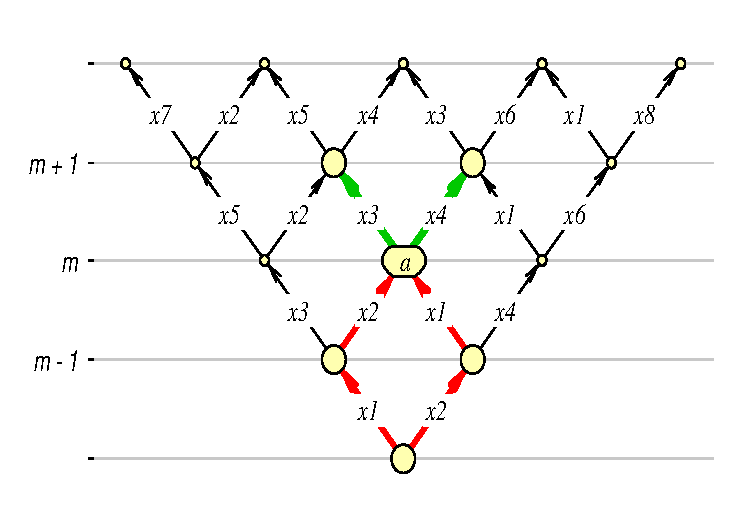
\includegraphics[width=77mm,height=44mm]{SC-graph-3a.eps}
    \caption{The SC-graph over 2-dimensional monotonic lattice of altitude~4.
        Algorithm $a$ at $m$-th layer has
        prohibitive subset $\{x1, x2\}$ and protective subset $\{x3, x4\}$.}
    \label{fig:SC-graph-3a}
\end{figure}

Figure\,\ref{fig:SC-graph-3a} shows an example of 2-dimensional lattice of altitude 4.
Like monotonic chain,
\mbox{SC-bound} for this model set is exact and easily follows from the common SC-bound.

\begin{lemma}
\label{lem:lattice-objects}
    There are only three types of objects in the set~$\XX$:

    1)~$m$~objects on which any classifier gives an error;\;

    2)~$Hh$~objects
    $\bigl\{x_t^d\colon t=0,\ldots,H{-}1,\, d=1,\ldots,h \bigr\}$
    such that
    $I(a_J,x_t^d) = \bigl[ t<j_d \bigr]$
    for any $|J| \leq H$;

    3)~other objects on which no classifier gives an error.
\end{lemma}
The proof is not difficult but needs a number of details, therefore we~omit it for reasons of space.

\begin{lemma}
\label{lem:lattice-exact}
    If $\mu$ is pessimistic ERM, then
    $\bigl[ \mu X {=} a_J \bigr] =
        \bigl[ X_J \subseteq X \bigr]
        \bigl[ X'_J \subseteq \X \bigr]$
    for all $a_J\in A$, where
    \begin{align*}
        X_J &= \bigl\{x_t^d\colon t=j_d,\; d=1,\ldots,h\bigr\}
        \text{~ is the protective subset;}
    \\
        X'_J &= \bigl\{x_t^d\colon t<j_d,\; d=1,\ldots,h\bigr\}
        \text{~ is the prohibitive subset.}
    \end{align*}
\end{lemma}
\begin{proof}
    Let us prove that if $X_J \subseteq X$ and $X'_J \subseteq \X$,
    then only the classifier~$a_J$
    can be an output of the learning algorithm: $\mu X = a_J$.

    The classifier~$a_J$ makes errors
    only on objects from~$X'_J$ all belonging to~$\X$;
    then $n(a_J,X)=0$.

    Consider a~classifier $a_K$ such that $K\not\leq J$.
    This means that $k_d > j_d$ for some coordinate~$d$.
    Then the classifier~$a_K$ produces an~error on the object~$x^d_{j_d}$
    that belongs to~$X_J$ and hence to~the~training sample~$X$.
    Therefore, the learning algorithm~$\mu$ being empirical risk minimizer
    will not choose~$a_K$.

    Consider a~classifier $a_K$ such that $K < J$.
    Then both $a_J$ and~$a_K$ do not make errors on the~training sample~$X$.
    Assume that $k_d < j_d$ for some coordinate~$d$.
    Then only $a_J$ makes an~error  on a~testing object~$x^d_{k_d}$.
    Therefore learning algorithm~$\mu$ being pessimistic
    will not choose~$a_K$.

    Thus, only the classifier~$a_J$ can be an output of the learning algorithm.
\end{proof}

\begin{theorem}
\label{th:lattice}
    If the learning algorithm~$\mu$ is~pessimistic ERM,
    the set~$A$ is a monotonic $h$-dimensional lattice of classifiers with altitude $H$
    and $m+Hh \leq L$, then
    \[
        Q_\eps(\mu,\XX)
        =
        \sum_{t=0}^{\min\{H,k\}}
            \CC_{h+t-1}^t \frac{\CC_{L-q-t}^{\ell-q}}{\CC_{L}^{\ell}}
            \Hyper{L-q-t}{m}{\ell-q}{\tfrac\ell L (m+t - \eps k)},
        \quad
        q=[t{<}H] h.
    \]
\end{theorem}
\begin{proof}
    Let us numerate nonempty layers of the monotonic lattice by $t=0,\ldots,H$.
    Note that $n(a_J) = m+t$ and $t=|J|$ for any classifier $a_J\in A$.

    It follows from lemma~\ref{lem:lattice-objects} that
    $r(a_J)=t$ and $q(a_J)=h$ for all $a_J \in A$
    except for classifiers from the last (highest) layer
    which do not have protective objects:
    $q(a_J) = 0$, $|J|=H$.

    All classifiers $a_J$ from one layer $t=|J|$
    have equal characteristics $q$, $r$, and $n$.
    Therefore, the sum over classifiers in~\eqref{eq:SC-bound}
    can be transformed into the sum over layers $t=0,\ldots,H$,
    with multiplier $|A_{m+t}| = \CC_{h+t-1}^t$ under the sum.

    By~lemma~\ref{lem:lattice-exact}
    the inequality~\eqref{eq:hyp1} transforms into the equality
    and gives a necessary and sufficient condition for $\mu X=a$.
    Then, the SC-bound~\eqref{eq:SC-bound} also transforms into the equality.
\end{proof}

In~a particular case, when $h=1$, the bound for monotonic lattice transforms into the bound for monotonic chain.
Both theoretical and experimental analysis of monotonic lattices can be found in~\cite{botov11pria}.
The purpose of this section is to show that
exact bounds can be obtained from the common SC-bound for nontrivial sets of classifiers.

%\TODO{
%    Chart.\\
%    UC-bound and SC-bound for monotine lattice of dimensions $d=2$ and $d=10$,
%    compared with Monte-Carlo estimations of probability of overfitting
%    for pessimistic ERM and discrepancy maximization,
%}
%
%\TODO{
%    Chart.\\
%    Computations show that contributions of layers decrease exponentially by~$t$,
%    so that only 5--10 lower layers are significant.
%}

\section{Tight SC-bound for threshold conjunctive rule}
\label{sec:RuleLearning}

Rule induction is a~well known, deeply studied, and widely used paradigm in~machine learning
\cite{rivest87learning,cohen99simple,marchand05learning,furnkranz05rocnrule,ruckert08experimental}.

\paragraph{Conjunctive rules.}
Consider a classification problem with labels $y_i\in\YY$, $i=1,\ldots,L$
assigned to each object $x_i\in\XX$ respectively.
Consider a parametric set~$R$ of \emph{conjunctive rules}
\begin{equation}
\label{eq:ConjRule}
    r(x; \theta) = \prod_{j\in J} \bigl[ x^j \leq \theta^j \bigr],
\end{equation}
where  $x=(x^1,\ldots,x^n)$ is a vector of numerical features of an object~$x$,
${J\subseteq \{1,\ldots,n\}}$ is a subset of features,
${\theta^j \in \RR}$ is a~threshold parameter for $j$-th feature.
Note that~\eqref{eq:ConjRule} can be easily generalized to
rules with conditions $\theta_1^j \leq x^j \leq \theta_2^j$ or $x^j \geq \theta^j$
simply by adding a~negated feature~$-x^j$.

An~object~$x$ is said to be \emph{covered} by the rule~$r$ if $r(x)=1$.

\paragraph{Rule learning.}
The rule induction system usually learns a rule set $R_y$ for each class $y\in\YY$ from a~training set~$X$.
Two criteria are optimized simultaneously to select useful rules~---
the number of positive and negative examples covered by~$r$, respectively:
\begin{align*}
    p(r,X)
    &=
    \#\bigl\{
        x_i\in X
    \bigm|
        r(x_i)=1,\; y_i=y
    \bigr\}
    \to\max;
\\
    n(r,X)
    &=
    \#\bigl\{
        x_i\in X
    \bigm|
        r(x_i)=1,\; y_i\neq y
    \bigr\}
    \to\min.
\end{align*}

In practice the two-criteria optimization task is reduced
to one-criterion task by means of heuristic function $H(p,n)$.
Examples of~$H$ are entropy, Gini index, Fisher's exact test, $\chi^2$- and $\omega^2$-tests,
and many others~\cite{furnkranz05rocnrule}.

\paragraph{Rule based classifier.}
After learning the rule sets~$R_y$ for all~$y\in\YY$
the classifier can be build~up as a composition of rules.
The weighted voting is a~most popular choice:
\[
    a(x) = \arg\max_{y\in \YY} \sum_{r\in R_y} w_r r(x),
\]
where weights $w_r \geq 0$ are to be learned from the training set~$X$.
So,~there are three things to learn:

1)~thresholds $\theta^j$,\: $j\in J$  for each subset~$J$;\;

2)~feature subset~$J$  for each rule~$r$;\;

3)~weight~$w_r$  for each rule~$r$.

Respectively, there are three reasons for overfitting.
In~this work we deal with overfitting resulting from thresholds learning
and use the SC-bound to build a~new criterion for feature subsets selection.
So,~our goal is to reduce overfitting for learning stages 1)~and~2),
with motivation that a~good classifier can be hardly build~up from overfitted rules.
We~leave the stage~3) beyond the scope of this paper
bearing in mind that the overfitting of weighted voting
is~now well understood~\cite{schapire97boosting,koltchinskii01further}.

\paragraph{The main idea of heuristic modification}
is to obtain the SC-bound on~both $p$ and~$n$ for a~fixed~$J$;
then to~get inverted estimates that hold with probability at least $1-\eta$:
\begin{align*}
    \tfrac 1k p(r,\X) & \geq \tfrac 1\ell p(r,X) - \eps_p(\eta),\\
    \tfrac 1k n(r,\X) & \leq \tfrac 1\ell n(r,X) + \eps_n(\eta),
\end{align*}
and substitute these estimates instead of $p,n$ in a heuristic function:
\[
    H'(p,n) =
    H \bigl(
        p - \ell \eps_p(\eta) ,
        n + \ell \eps_n(\eta)
    \bigr).
\]

The modified heuristic~$H'$ estimates the quality of~a~rule
with a~fixed subset of features~$J$ and learnt thresholds.
Both discrepancies $\eps_p(\eta)$ and $\eps_n(\eta)$
are very sensitive to the number of rules in bottom levels of the SC-graph.
The more rules the bottom levels contain, the higher is overfitting.
The modified heuristic~$H'$ can be considered
as a~feature selection criterion based on a~data-dependent generalization bound.

\medskip
In~order to specialize the SC-bound for conjunctive rules
we first define the binary loss function:
$I(r,x_i) = \bigl[ r(x_i) \neq [y_i\!=\!y] \bigr]$,\; $i=1,\ldots,L$,
for any rule~$r$ of class~$y$.
Second, we will describe how to iterate in~\eqref{eq:SC-bound}
only rules having pairwise different error vectors.
As~a~result we will obtain
a~heuristic function~$H$ modified by the SC-bound
which can be easily incorporated into any rule inducer.

\paragraph{Classes of equivalent rules.}

Fig.\,\ref{fig:sample10}(a) shows an~example of two-dimensional objects set~$\XX$
combining the scatter plot of initial objects with the set $R$ of rules
$r(x;\theta) =[x^1\leq \theta^1]\,[x^2\leq\theta^2]$.
Each object and each rule is represented
by a~node of ${(L+1)\times(L+1)}$ grid in coordinate plane $\theta^1,\theta^2$.
Nodes containing the rules with equal error vectors are connected.
Fig.\,\ref{fig:sample10}(b)
shows the same objects set,
but only representative rules (with pairwise different error vectors) are left on the plot.
Rules with Hamming distance~1 are connected.
Fig.\,\ref{fig:sample10}(c)
shows the SC-graph of the rule set  isomorphic to the graph
on~Fig.\,\ref{fig:sample10}(b).

From the above example it seems that the equivalence classes of rules have a~nontrivial structure.
In fact, this is not the case and equivalence classes can be efficiently described and searched.

\begin{figure}[t!]
    \noindent\centering
    \raisebox{10mm}{(a)}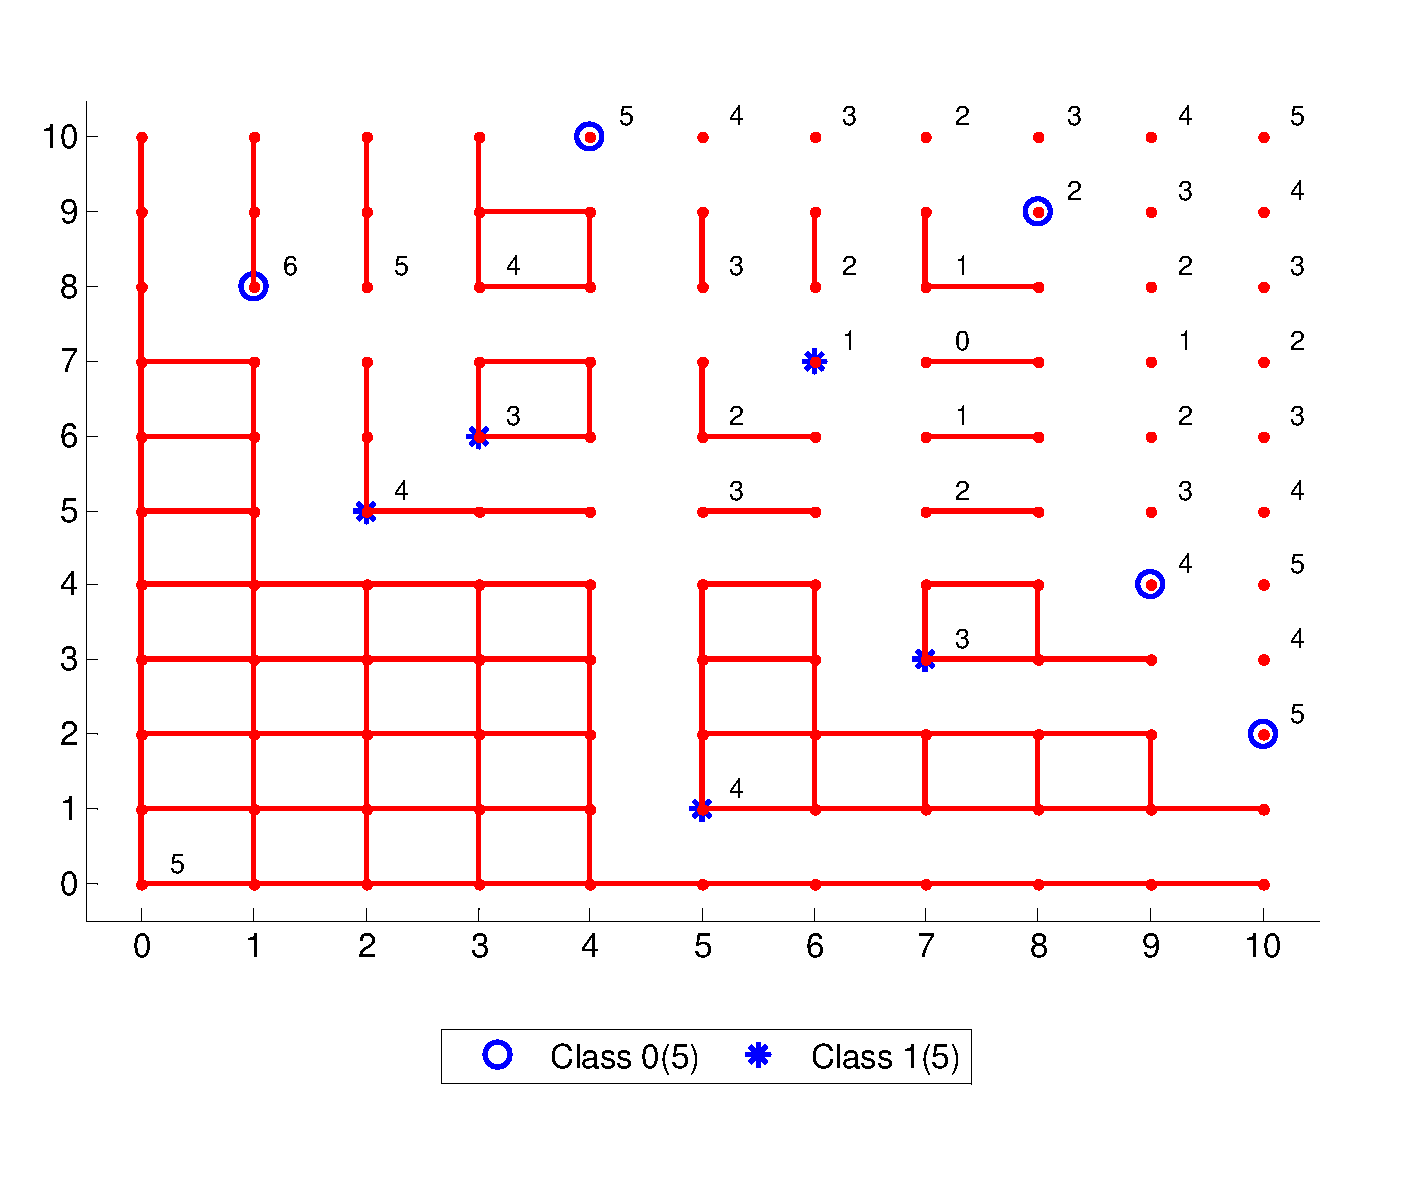
\includegraphics[width=70mm]{ivahnenko-correctAlgorithm.eps}
    \raisebox{10mm}{(b)}\raisebox{2mm}{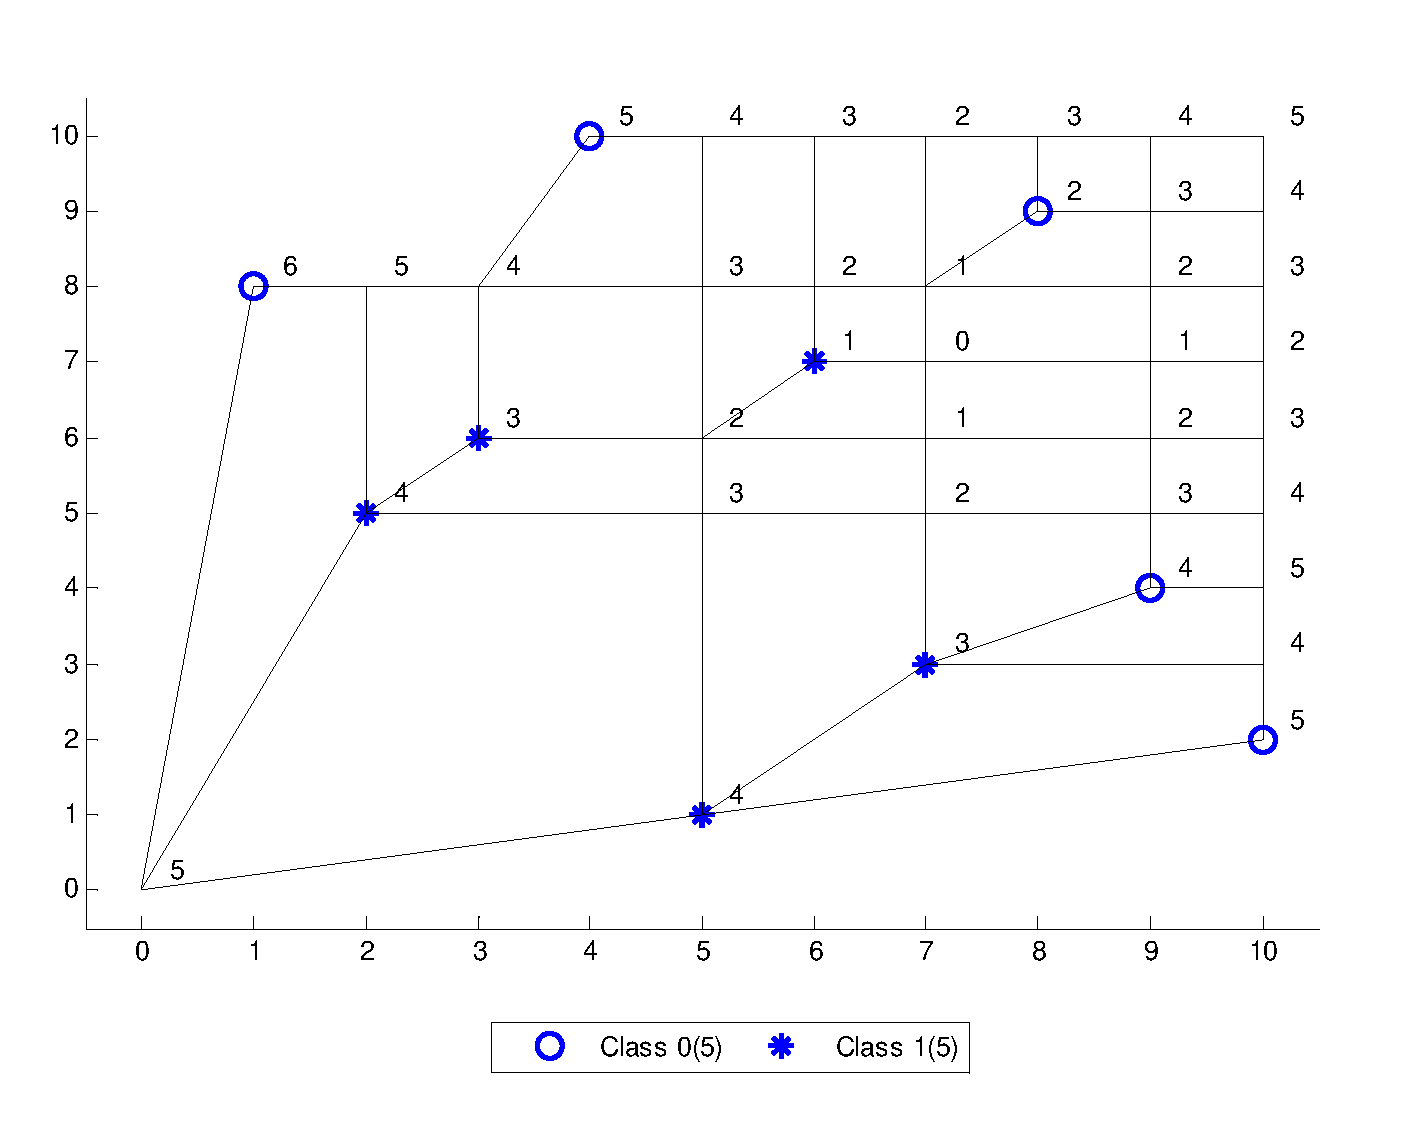
\includegraphics[width=70mm]{ivahnenko-Links.eps}}\\
    (c)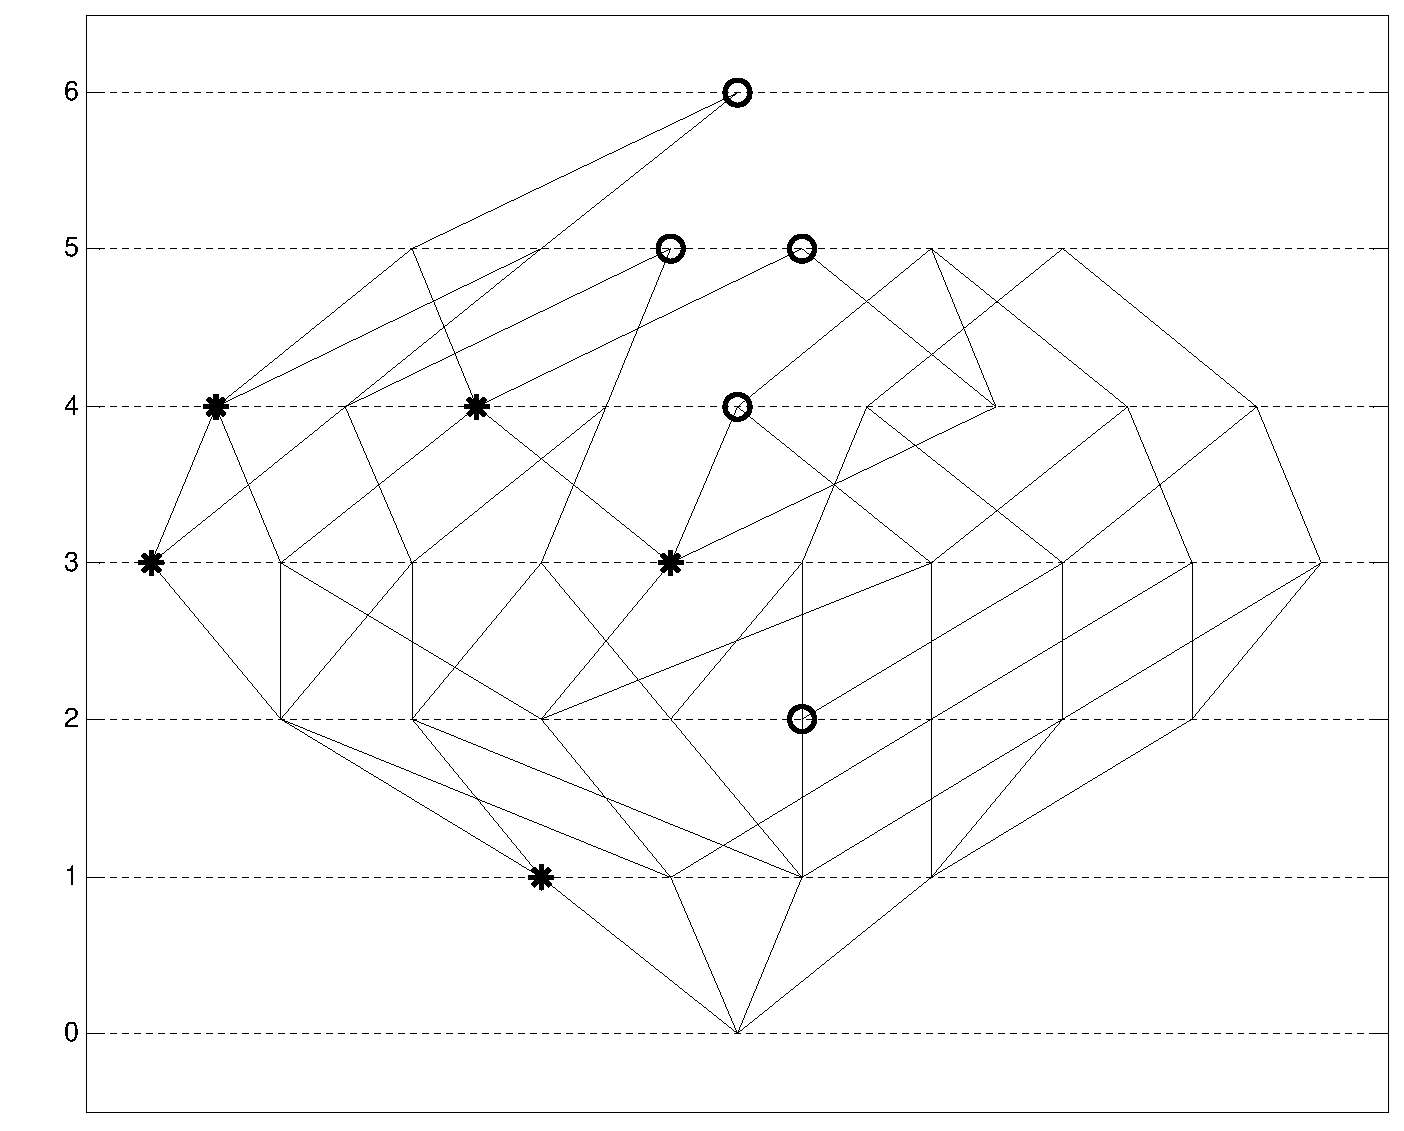
\includegraphics[width=70mm]{ivahnenko-LinksTree.eps}
    \caption{Example of a set of $L = 10$ objects of two classes~(a),
        the graph of representative rules~(b),
        and the SC-graph~(c).}
    \label{fig:sample10}
\end{figure}

For the sake of simplicity consider a~case when
all values $x_i^j$, $i=1,\ldots,L$ are pairwise different
for each feature $j=1,\ldots,n$.
Without loss of generality, assume that the features take integer values $1,\ldots,L$
and the thresholds take integer values $0,\ldots,L$.

The loss function~$I$ induces an equivalence relation on the set of rules~$R$.
Two rules are equivalent, $r\sim r'$ if their error vectors are equal.
Let
${u=(u^j)_{j\in J}}$, ${v=(v^j)_{j\in J}}$
be a pair of vectors.
Define a~partial order relation
${(u\leq v) \;\leftrightarrow\; \forall j\in J\; (u^j \leq v^j)}$.
Define
${(u < v) \;\leftrightarrow\; (u\leq v}$ and ${u\neq v)}$.

By $\theta^j_r$ denote a value of threshold on $j$-th feature for a rule $r(x;\theta)$ ,
$\theta = (\theta^j_r)_{j\in J}$

\begin{lemma}
\label{lem:theta_E}
    If ${E \subseteq R}$ is equivalence class of rules,
    then a~rule $r(x;\theta_E)$
    belongs to the equivalence class~$E$,
    where
    $\theta_E^j = \min\limits_{r\in E} \theta^j_r$.
\end{lemma}
\begin{proof}
    All equivalent rules $r\in E$ have equal binary error vectors.
    Then a~binary function
    \[
        r_E(x) = \prod\limits_{r\in E} r( x; \theta_r )
    \]
    takes the same value on each object ${x\in\XX}$ as~any rule~$r$ from~$E$,
    ${r_E(x) = r(x; \theta_r)}$.
    Moreover, the binary function $r_E$ can be represented in the form~\eqref{eq:ConjRule},
    so it is also a~rule:
    \[
        r_E(x)
        =
        \prod_{r\in E}
            \prod_{j\in J}
            \bigl[ x^j\leq \theta^j_r \bigr]
        =
        \prod_{j\in J}
            \bigl[ x^j\leq \min_{r\in E} \theta^j_r \bigr]
        =
        \prod_{j\in J}
            \bigl[ x^j\leq \theta^j_E \bigr]
        = r(x;\theta_E).
    \]
    This means that the rule $r(x;\theta_E)$ pertains to the equivalence class~$E$.
\end{proof}

The rule $r_E(x) \equiv r(x;\theta_E)$ from the previous lemma will be called
a~\emph{representative rule} of the equivalence class~$E$.
On~figure\,\ref{fig:sample10}
representative rules correspond to~lower left corners of~equivalence classes:
$(0,0)$, $(1,8)$, $(2,5)$, $(5,1)$, etc.

A \emph{boundary point} of the subset~$S\subseteq \XX$ is a~vector~$\theta_S$ with coordinates
$\theta^j_S = \max\limits_{x\in S} x^j$,\;
$j\in J$.

A \emph{boundary object} of the subset~$S\subseteq \XX$ is any object $x\in S$ such that $x^j = \theta_S^j$ for some~$j$.

A \emph{boundary subset} is a~subset~$S\subseteq \XX$ such that all objects ${x\in S}$ are boundary objects of~$S$.

Empty set is assumed to be a~boundary subset with boundary point $\theta^j_{\emset}=0$, $j\in J$.

Note that $r(x,\theta_S) = 1$ for any $x\in S$.

\begin{lemma}
\label{lem:BoundarySubset}
    If a~threshold vector~$\theta$ is a~boundary point of some boundary subset,
    then this subset can be unambiguously determined by the threshold vector~$\theta$:
    \begin{equation}
    \label{eq:BoundarySubset}
        S_\theta =
        \bigcup_{j\in J}
        \bigl\{
            x\in\XX
        \bigm|
            x^j = \theta^j,\;
            r(x,\theta) = 1
        \bigr\}.
    \end{equation}
\end{lemma}
\begin{proof}
    If~${\theta = \theta_\emset}$, then ${S_\theta=\emset}$ by~definition.
    Otherwise,
    threshold vector $\theta$ is~a~boundary point,
    and
    for any index ${j\in J}$ an~object ${x\in \XX}$ exists such that
    ${x^j = \theta^j}$ and
    ${x^{\bar\jmath} \leq \theta^{\bar\jmath}}$ for all other indices ${\bar\jmath \in J\setminus \{j\}}$.
    Then  $r(x,\theta) = 1$,
    and it~follows from~\eqref{eq:BoundarySubset} that $x\in S_\theta$.
    The index ${j\in J}$ was chosen arbitrarily.
    Therefore, the threshold vector~$\theta$ is~a~boundary point of the subset~$S_\theta$.
    The subset~$S_\theta$ is~a boundary because
    each of its objects is~a boundary according to~\eqref{eq:BoundarySubset}.
\end{proof}

\begin{theorem}
\label{th:thetaE=thetaS}
    Each equivalence class~$E$ bijectively corresponds
    to~a~boundary subset~$S$: $\theta_E = \theta_S$.
\end{theorem}
\begin{proof}
    Consider an~arbitrary equivalence class~$E$ with representative rule $r(x;\theta_E)$.
    By~lemma~\ref{lem:theta_E} the decrease of threshold~$\theta^j_E$ along any coordinate ${j\in J}$
    changes the value~$r(x;\theta_E)$ on~some object~$x\in\XX$ such that $x\leq \theta_E$.
    This value may only be decreased:
    ${[x^j \leq \theta^j_E] = 1}$,\;
    ${[x^j \leq \theta^j_E-1] = 0}$.
    From this it follows that
    ${x^j = \theta^j_E}$,
    then $x$~is~a~boundary object in the subset
    ${\bigl\{ x'\in\XX \colon x'\leq \theta_E\bigr\}}$.
    As~feature~$j$ is~arbitrary, this means that
    threshold vector $\theta_E$ is~a~boundary point.
    According to lemma~\ref{lem:BoundarySubset} it determines a~unique boundary subset.

    The converse is also true.
    Any~boundary subset~$S$ has a~boundary point~$\theta_S$.
    The rule $r(x;\theta_S)$ is a~representative rule of the equivalence class~$E$ to which it belongs,
    because the decrease of~the threshold $\theta^j_S$ along any coordinate ${j\in J}$
    changes the value $r(x;\theta_S)$ on~some boundary object of the subset~$S$.

    Thus we~conclude that each equivalence class~$E$ bijectively corresponds
    to~a~boundary subset~$S$ such that $\theta_E = \theta_S$.
\end{proof}

%\paragraph{Properties of boundary subsets.}
Denote~$M_q$ the set of all boundary subsets of size~$q$
and recapitulate its properties:

\medskip
1) $M_1$ consists of all $L$ one-element subsets, $M_1 = \bigl\{ \{x_1\},\ldots,\{x_L\} \bigr\}$;

\nopagebreak
2) $M_2$ consists of all pairs of incomparable objects from~$\XX$;

3) the size of boundary subset can not exceed the rank of conjunction:
$M_q = \emset$ for all $q>|J|$;

4) any boundary subset consists of pairwise incomparable objects;
the converse is not obligatory true:
a~subset of three or more pairwise incomparable objects may not be a~boundary subset;

5) any subset ${S'\subset S}$ of the boundary subset~$S$ is a~boundary subset too.

\medskip
A~simple algorithm which iterates all boundary subsets follows from these properties.
At~the first step
a~subset~$M_1$ is~formed from all $L$ one-object subsets.
At~each subsequent step $q=2,\ldots,|J|$
for all subsets ${S'\in M_{q-1}}$ and for all objects $x \in \XX \setminus S'$
if the subset $S = S'\cup\{x\}$ is~boundary (which can be easily tested by~definition),
then $S$~joins~$M_q$.

More efficient but more complicated level-wise algorithm for SC-bound calculation
is~described in~\cite{voron11premi}.
It~iterates rules from bottom to upper levels
and uses early stopping to bypass rules
that do not make significant contribution to the SC-bound.
Additionally this algorithm calculates the connectivity and the inferiority of each rule.

\begin{table}[t]
    \def\r#1{\textbf{#1}}
    \caption{Experimental results on 6 real data sets from UCI Machine Learning Repository.
        For each pair $\langle$task, algorithm$\rangle$
        an~average testing error obtained from 10-fold cross validation is~given, in~percents.
        For each task three best results are bold-emphasized.
        Algorithms 1--7 are baseline rule learners.
        Our~algorithms:
        WV~---~Weighted Voting,\;
        DL~---~Decision List,\;
        SC~---~using heuristic modified by SC-bound,\;
        MC~---~using heuristic modified by Monte-Carlo estimation of overfitting.
    }
    \label{tab:Experiment}
    \medskip\centering
    \begin{tabular}{|r|l||c|c|c|c|c|c|}
        \hline
        && \multicolumn{6}{c|}{tasks} \\
        \cline{3-8}
        & \raisebox{1.2ex}{algorithms}
                & australian  & echo-card  & heart dis.   & ~hepatitis~   & ~~~labor~~~   & ~~~liver~~~  \\
        \hline
        1& RIPPER$-$opt &15.5&\r{2.9}&19.7&20.7&18.0&32.7\\
        \hline
        2& RIPPER$+$opt &15.2&5.5&20.1&23.2&18.0&\r{31.3}\\
        \hline
        3& C4.5 (Tree) &14.2&5.5&20.8&18.8&14.7&37.7\\
        \hline
        4& C4.5 (Rules)&15.5&6.8&20.0&18.8&14.7&37.5\\
        \hline
        5& C5.0       &\r{14.0}&4.3&21.8&20.1&18.4&31.9\\
        \hline
        6& SLIPPER    &15.7&4.3&\r{19.4}&\r{17.4}&\r{12.3}&32.2\\
        \hline
        7& LR         &14.8&4.3&19.9&18.8&14.2&32.0\\
        \hline
        \hline
        8& WV         &14.9&4.3&20.1&19.0&14.0&32.3\\
        \hline
        9& DL         &15.1&4.5&20.5&19.5&14.7&35.8\\
        \hline
        \hline
        10& \r{WV$+$MC}      &\r{13.9}&\r{3.0}&\r{19.5}&\r{18.3}&\r{13.2}&\r{30.7}\\
        \hline
        11& \r{DL$+$MC}      &14.5&3.5&19.8&18.7&13.8&32.8\\
        \hline
        \hline
        12& \r{WV$+$SC}     &\r{14.1}&\r{3.2}&\r{19.3}&\r{18.1}&\r{13.4}&\r{30.2}\\
        \hline
        13& \r{DL$+$SC}     &14.4&3.6&19.5&18.6&13.6&32.3\\
        \hline
    \end{tabular}
\end{table}

\paragraph{Experiment.}
We use state-of-the art algorithms
C4.5~\cite{quinlan96bagging},
C5.0~\cite{quinlan93programs},
\mbox{RIPPER}~\cite{cohen95fast}, and
\mbox{SLIPPER}~\cite{cohen99simple}
as~baseline rule learners.
Our~rule learning engine is~based on breadth-first search as~features selection strategy.
Fisher's exact test~\cite{martin97exact} is~used as~heuristic~$H$.
To~build compositions of rules we use three algorithms.
Logistic Regression~(LR) is a~linear classifier that aggregates rules learned independently.
Weighted Voting~(WV) is a~boosting-like ensemble of rules, similar to~\mbox{SLIPPER},
which trains each next rule on~reweighted training set.
Decision List~(DL) is~a~greedy algorithm,
which trains each next rule on~training objects not covered by all previous rules.

There are two modifications of~heuristic~$H'(p,n)$.
The~SC-modification uses SC-bound on the probability of~overfitting~$Q_\eps$ as~described above.
The~MC-modification uses the Monte-Carlo estimation of~$Q_\eps$
via 100~random partitions $\XX = X\sqcup\X$.
For both modifications we set $\ell=k$.

Table~\ref{tab:Experiment} shows that
initially our algorithms WV, DL are comparable to the baseline.
WV~outperforms DL, which corresponds to the results of other authors.
Both SC- and MC- modifications reduce overfitting significantly
and always outperform their respective initial versions.
The~difference between SC- and MC- modifications is not significant.
Then, a~moderate looseness of~the SC-bound does not reduce %prevent
its practical usefulness as~a~rule selection criterion.

\section{Conclusion}

Splitting and connectivity (SC) are very important data-dependent properties
of a~set of classifiers that determines its generalization ability.
This work gives a~combinatorial SC-bound on the probability of overfitting.
The SC-bound takes into account both the learning algorithm
and a~fine internal structure of the set of~classifiers
represented by the SC-graph.
The SC-bound can be exact (non-asymptotical, non-overestimated)
for some nontrivial sets of classifiers like
the monotonic chain and
the multidimensional monotonic lattice.

If the discrepancy maximization is~considered as~a~learning algorithm,
then the SC-bound transforms into the UC (uniform connectivity) bound
and gives the probability of a~large uniform deviation.
Thus, the UC-bound can be used for the Rademacher complexity estimation.
Note that the UC-bound takes into account the connectivity but neglect the splitting.

The~SC-bound being applied to threshold conjunctive rules
helps to~select features for each rule more accurately,
and then to~reduce overfitting of a~rule induction machine.
In~practice this can be implemented as a~slight modification
of~a~heuristic function which estimates the usefulness of a~rule.
Experiments on six real data sets show that
the proposed modification reduces overfitting.

%\def\url#1{}
%\bibliography{MachLearn}

\begin{thebibliography}{27}
\providecommand{\natexlab}[1]{#1}
\providecommand{\url}[1]{\texttt{#1}}
\expandafter\ifx\csname urlstyle\endcsname\relax
  \providecommand{\doi}[1]{doi: #1}\else
  \providecommand{\doi}{doi: \begingroup \urlstyle{rm}\Url}\fi

\bibitem[Botov(2011)]{botov11pria}
    P.~V.~Botov.
    \newblock Exact bounds on probability of overfitting for multidimensional model sets of classifiers (to~appear).
    \newblock \emph{Pattern Recognition and Image Analysis}, 2011.
\bibitem[Boucheron et~al.(2000)Boucheron, Lugosi, and Massart]{boucheron00sharp}
    S.~Boucheron, G.~Lugosi, and P.~Massart.
    \newblock A sharp concentration inequality with applications.
    \newblock \emph{Random Structures and Algorithms}, 16\penalty0 (3):\penalty0 277--292, 2000.
\bibitem[Boucheron et~al.(2005)Boucheron, Bousquet, and Lugosi]{boucheron05theory}
    S.~Boucheron, O.~Bousquet, and G.~Lugosi.
    \newblock Theory of classification: A survey of some recent advances.
    \newblock \emph{ESAIM: Probability and Statistics}, \penalty0 (9):\penalty0 323--375, 2005.
\bibitem[Cohen(1995)]{cohen95fast}
    W.~W.~Cohen.
    \newblock Fast effective rule induction.
    \newblock In \emph{Proc. of the 12th International Conference on Machine Learning, Tahoe City, CA}, pages 115--123. Morgan Kaufmann, 1995.
\bibitem[Cohen and Singer(1999)]{cohen99simple}
    W.~W.~Cohen and Y.~Singer.
    \newblock A simple, fast and effective rule learner.
    \newblock In \emph{Proc. of the 16 National Conference on Artificial Intelligence}, pages 335--342, 1999.
\bibitem[F\"urnkranz and Flach(2005)]{furnkranz05rocnrule}
    J.~F\"urnkranz and P.~A.~Flach.
    \newblock Roc `n' rule learning-towards a better understanding of covering algorithms.
    \newblock \emph{Machine Learning}, 58\penalty0 (1):\penalty0 39--77, 2005.
\bibitem[Graham et~al.(1994)Graham, Knuth, and Patashnik]{knuth98concrete-eng}
    R.~L.~Graham, D.~E.~Knuth, and O.~Patashnik.
    \newblock \emph{Concrete Mathematics}.
    \newblock Reading, Massachusetts: Addison-Wesley, 1994.
\bibitem[Haussler et~al.(1994)Haussler, Littlestone, and Warmuth]{haussler94predicting}
    D.~Haussler, N.~Littlestone, and M.~K. Warmuth.
    \newblock Predicting $\{0,1\}$-functions on randomly drawn points.
    \newblock \emph{Inf. Comput.}, 115:\penalty0 248--292, December 1994.
\bibitem[Koltchinskii et~al.(2001)Koltchinskii, Panchenko, and Lozano]{koltchinskii01further}
    V.~Koltchinskii, D.~Panchenko, and F.~Lozano.
    \newblock Further explanation of the effectiveness of voting methods: {T}he game between margins and weights.
    \newblock In \emph{14th Annual Conference on Computational Learning Theory,
      {COLT} 2001 and 5th {E}uropean Conference on Computational Learning Theory,
      {EuroCOLT} 2001, Amsterdam, The Netherlands, July 2001, Proceedings}, volume 2111, pages 241--255.
      Springer, Berlin, 2001.
\bibitem[Langford(2002)]{langford02quantitatively}
    J.~Langford.
    \newblock \emph{Quantitatively Tight Sample Complexity Bounds}.
    \newblock PhD thesis, Carnegie Mellon Thesis, 2002.
\bibitem[Lugosi(2003)]{lugosi98concentrationmeasure}
    G.~Lugosi.
    \newblock On concentration-of-measure inequalities.
    \newblock Machine Learning Summer School, Australian National University, Canberra, 2003.
\bibitem[Marchand and Sokolova(2005)]{marchand05learning}
    M.~Marchand and M.~Sokolova.
    \newblock Learning with decision lists of data-dependent features.
    \newblock \emph{Journal of Machine Learning Reasearch}, 6:\penalty0 427--451, 2005.
\bibitem[Martin(1997)]{martin97exact}
    J.~K.~Martin.
    \newblock An exact probability metric for decision tree splitting and stopping.
    \newblock \emph{Machine Learning}, 28\penalty0 (2-3):\penalty0 257--291, 1997.
\bibitem[Philips(2005)]{philips05datadependent}
    P.~Philips.
    \newblock \emph{Data-Dependent Analysis of Learning Algorithms}.
    \newblock PhD thesis, The Australian National University, Canberra, 2005.
\bibitem[Quinlan(1993)]{quinlan93programs}
    J.~R.~Quinlan.
    \newblock \emph{C4.5: Programs for machine learning}.
    \newblock Morgan Kaufmann, San Francisco, CA, 1993.
\bibitem[Quinlan(1996)]{quinlan96bagging}
    J.~R.~Quinlan.
    \newblock Bagging, boosting, and {C4.5}.
    \newblock In \emph{{AAAI}/{IAAI}, Vol. 1}, pages 725--730, 1996.
\bibitem[Rivest(1987)]{rivest87learning}
    R.~L. Rivest.
    \newblock Learning decision lists.
    \newblock \emph{Machine Learning}, 2\penalty0 (3):\penalty0 229--246, 1987.
\bibitem[R\"uckert and Raedt(2008)]{ruckert08experimental}
    U.~R\"uckert and L.~De~Raedt.
    \newblock An experimental evaluation of simplicity in rule learning.
    \newblock \emph{Artif. Intell.}, 172\penalty0 (1):\penalty0 19--28, 2008.
\bibitem[Schapire et~al.(1998)Schapire, Freund, Lee, and Bartlett]{schapire97boosting}
    R.~E.~Schapire, Y.~Freund, We~Sun Lee, and P.~Bartlett.
    \newblock Boosting the margin: a new explanation for the effectiveness of  voting methods.
    \newblock \emph{Annals of Statistics}, 26\penalty0 (5):\penalty0 1651--1686, 1998.
\bibitem[Sill(1998)]{sill98phd}
    J.~Sill.
    \newblock \emph{Monotonicity and connectedness in learning systems}.
    \newblock PhD thesis, California Institute of Technology, 1998.
\bibitem[Vapnik and Chervonenkis(1971)]{vapnik71uniform-eng}
    V.~N.~Vapnik and A.~Ya.~Chervonenkis.
    \newblock On the uniform convergence of relative frequencies of events to their probabilities.
    \newblock \emph{Theory of Probability and its Applications}, 16\penalty0 (2):\penalty0 264--280, 1971.
\bibitem[Vapnik(1998)]{vapnik98stat}
    V.~N.~Vapnik.
    \newblock \emph{Statistical Learning Theory}.
    \newblock Wiley, New York, 1998.
\bibitem[Vayatis and Azencott(1999)]{vayatis99distributiondependent}
    N.~Vayatis and R.~Azencott.
    \newblock Distribution-dependent {Vapnik-Chervonenkis} bounds.
    \newblock \emph{Lecture Notes in Computer Science}, 1572:\penalty0 230--240, 1999.
\bibitem[Vorontsov(2008)]{voron08pria-eng}
    K.~V.~Vorontsov.
    \newblock Combinatorial probability and the tightness of generalization bounds.
    \newblock \emph{Pattern Recognition and Image Analysis}, 18\penalty0 (2):\penalty0 243--259, 2008.
\bibitem[Vorontsov(2009)]{voron09roai2008}
    K.~V.~Vorontsov.
    \newblock Splitting and similarity phenomena in the sets of classifiers and their effect on the probability of overfitting.
    \newblock \emph{Pattern Recognition and Image Analysis}, 19\penalty0 (3):\penalty0 412--420, 2009.
\bibitem[Vorontsov(2010)]{voron10pria-eng}
    K.~V.~Vorontsov.
    \newblock Exact combinatorial bounds on the probability of overfitting for empirical risk minimization.
    \newblock \emph{Pattern Recognition and Image Analysis}, 20\penalty0 (3):\penalty0 269--285, 2010.
\bibitem[Vorontsov and Ivahnenko(2011)]{voron11premi}
    K.~V.~Vorontsov and A.~A.~Ivahnenko.
    \newblock Tight combinatorial generalization bounds for threshold conjunction rules (to~appear).
    \newblock In \emph{4th International Conference on Pattern Recognition and Machine Intelligence (PReMI'11).
    June~27 -- July~1, 2011}, 2011.
\end{thebibliography}

\end{document}
